% Thesis Documentation Template for "MPGV monitor: Dynamic Visualisation of Seismic Data for Iceland"

\documentclass[12pt]{article}
\usepackage[a4paper]{geometry}
\geometry{margin=2.5cm}
\usepackage[skip=0.8em]{parskip}
\usepackage{lmodern}              % Latin Modern — matches official HÍ template
\usepackage{fixcmex}              % Fix Latin Modern large symbol math font sizing
\usepackage[utf8]{inputenc}
\usepackage[T1]{fontenc}
\usepackage[icelandic,english]{babel}
\usepackage{microtype}
\usepackage[svgnames]{xcolor}
\usepackage{titlesec}
\titlespacing{\section}{0ex}{*3}{*1}
\titlespacing{\subsection}{0ex}{*3}{*1}
\titlespacing{\subsubsection}{0ex}{*3}{*1}
\titlelabel{\thetitle\hspace{0.6em}}
% Sans-serif section headings — matches official HÍ template
\titleformat{\section}{\Large\sffamily\bfseries}{\thesection}{0.6em}{}
\titleformat{\subsection}{\large\sffamily\bfseries}{\thesubsection}{0.6em}{}
\titleformat{\subsubsection}{\normalsize\sffamily\bfseries}{\thesubsubsection}{0.6em}{}
\usepackage{graphicx}
\usepackage{minted}
\usemintedstyle{friendly}
\usepackage[leqno]{mathtools}
\usepackage{xfrac}
\usepackage[nice]{nicefrac}
\usepackage{booktabs}
\usepackage{caption}
\captionsetup{font={small,it}, labelfont={bf,it}, margin=2cm} % Italic captions — matches HÍ template
\usepackage{siunitx}
\usepackage{float}
\usepackage[shortlabels]{enumitem}
\usepackage{hyperref}
\hypersetup{
    colorlinks,
    linkcolor=DarkBlue,
    citecolor=DarkBlue,
    urlcolor=DarkBlue
}
% Package for headers and footers
\usepackage{fancyhdr}

\usepackage{csquotes}

% Header and Footer settings
\pagestyle{fancy}
\fancyhf{} % Clear default header/footer

% Header
\fancyhead[R]{MPGV Monitor: Dynamic Visualization of Seismic Data for Iceland} % Top-right header
\renewcommand{\headrulewidth}{0.4pt} % Add a line under the header

% Footer
\fancyfoot[C]{\thepage \\ \phantom{a}}
\fancyfoot[R]{\phantom{\thepage} \\ \small Faculty of Industrial Engineering, Mechanical Engineering and Computer}
\renewcommand{\footrulewidth}{0.4pt} % Add a line above the footer

% Exclude header and footer on the title page
\fancypagestyle{plain}{ % Redefine the plain page style (used by title page)
    \fancyhf{} % Clear header/footer for title page
    \renewcommand{\headrulewidth}{0pt} % Remove header rule
    \renewcommand{\footrulewidth}{0pt} % Remove footer rule
}

\usepackage[a4paper]{geometry}
\geometry{margin=2.5cm}
\usepackage{tikz}
\usetikzlibrary{shapes.geometric, arrows, arrows.meta, positioning}

\tikzstyle{startstop} = [rectangle, rounded corners, minimum width=3cm, minimum height=1cm,text centered, draw=black, fill=red!30]
\tikzstyle{process} = [rectangle, minimum width=3cm, minimum height=1cm, text centered, draw=black, fill=blue!30]
\tikzstyle{decision} = [diamond, minimum width=3cm, minimum height=1cm, text centered, draw=black, fill=green!30]
\tikzstyle{arrow} = [thick,->,>=stealth]

% HÍ brand colour (official corporate design)
\definecolor{hiblue}{RGB}{16,9,159}

% ============================ NEW COMMANDS =============================
\newcommand{\highlight}[1]{\textcolor{FireBrick}{#1}}
\newcommand{\code}[1]{\texttt{#1}}

% ============================ DOCUMENT START ============================
\begin{document}
\frenchspacing          % uniform word spacing — no extra gap after sentence periods

% Title Page (outer cover — official University of Iceland M.Sc. thesis style)
\begin{titlepage}
    \thispagestyle{empty}
    % --- TikZ overlay: official HÍ banner + bottom blue bar + faculty label ---
    \begin{tikzpicture}[remember picture, overlay]
        % Official HÍ banner image (full page width, anchored to top)
        \node[anchor=north west, inner sep=0pt] at (current page.north west)
            {
\includegraphics[width=\paperwidth]{Screenshots/banner.png}};
        % Bottom blue bar (full width, 10 mm tall)
        \node(bottom)[shape=rectangle, fill=hiblue, minimum height=10mm,
            minimum width=\paperwidth, anchor=south west]
            at (current page.south west) {};
        % Faculty name centred above the bottom bar
        \node[above=0.4cm of bottom] {
            \begin{tabular}{c}
                \sffamily\small\textcolor{hiblue}{\textbf{\MakeUppercase{
                Faculty of Industrial Engineering, Mechanical Engineering
                and Computer Science}}}
            \end{tabular}
        };
    \end{tikzpicture}

    \enlargethispage{3cm}
    \vspace*{3.5cm}

    % Centred minipage matching official HÍ template layout
    \newlength{\currentparskip}
    \setlength{\currentparskip}{\parskip}
    \hspace*{-2.7cm}%
    \begin{minipage}[t][20.0cm]{1.0\paperwidth}
        \setlength{\parskip}{\currentparskip}
        \begin{center}
            \vspace*{\stretch{1.5}}

            {\huge\sffamily\bfseries MPGV Monitor: Dynamic Visualization\\
            of Seismic Data for Iceland\par}

            \vspace{\stretch{1.0}}

            {\normalfont\Large\sffamily Muhammad Faheem Sajjad\par}

            \vspace*{\stretch{2.75}}

            {\normalfont\sffamily 2026\par}

            \vspace{\stretch{0.5}}

            {\normalfont\Large\sffamily M.Sc.\ thesis\\
            in Computer Science\par}

            \vspace*{\stretch{1.0}}
        \end{center}
    \end{minipage}
\end{titlepage}

% Blank page after cover
\clearpage
\null
\thispagestyle{empty}
\newpage

% Inner title page (detailed — official HÍ M.Sc. thesis style)
\begin{titlepage}
    \thispagestyle{empty}
    \begin{center}
        \vspace*{\stretch{0.5}}

        {\Large\sffamily\bfseries MPGV Monitor: Dynamic Visualization\\
        of Seismic Data for Iceland\par}

        \vspace*{\stretch{1.0}}

        {\sffamily Muhammad Faheem Sajjad\par}

        \vspace*{\stretch{1.0}}

        {\normalsize 60 ECTS thesis submitted in partial fulfillment of a\\
        \textit{Magister Scientiarum} degree in Computer Science\par}

        \vspace*{\stretch{1.0}}
        {\large\sffamily Supervisor\\}
        Kristján Jónasson\par

        \vspace*{\stretch{0.25}}
        {\large\sffamily Advisor\\}
        Esa Olavi Hyytiä\par

        \vspace*{\stretch{0.25}}
        {\large\sffamily M.Sc.\ Committee\\}
        Kristján Jónasson\\
        ...\par

        \vspace*{\stretch{0.25}}
        {\large\sffamily Examiner\\}
        ...\par
        
        \vspace*{\stretch{1.0}}

        Faculty of Industrial Engineering, Mechanical Engineering and Computer Science\\
        School of Engineering and Natural Sciences\\
        University of Iceland\\
        Reykjavik, 2026

        \vspace*{\stretch{0.5}}
    \end{center}
\end{titlepage}

% ============================ COLOPHON / COPYRIGHT PAGE ============================

\clearpage
\thispagestyle{empty}
\vspace*{\fill}
\renewcommand{\baselinestretch}{1.5}\normalsize
\sffamily{MPGV Monitor: Dynamic Visualization of Seismic Data for Iceland} \\
60 ECTS thesis submitted in partial fulfillment of a M.Sc.\ degree in Computer Science \\ \\
Faculty of Industrial Engineering, Mechanical Engineering and Computer Science \\
School of Engineering and Natural Sciences \\
University of Iceland \\
Dunhagi 5 \\
107, Reykjavik
Iceland \\
Telephone: 525 4000 \\ \\

\vspace*{\lineskip}

Bibliographic information: \\
Muhammad Faheem Sajjad (2026) \emph{MPGV Monitor: Dynamic Visualization of Seismic Data for Iceland}, M.Sc.\ thesis, Faculty of Industrial Engineering, Mechanical Engineering and Computer Science, University of Iceland.\\

Copyright \textcopyright~2026 Muhammad Faheem Sajjad \\
This thesis may not be copied in any form without author permission.\\

Reykjavik, Iceland, 2026 \\
\renewcommand{\baselinestretch}{1.0}\normalsize
\newpage

% ============================ MAIN CONTENT ============================

% Add a blank page
\clearpage
\null
\thispagestyle{empty} % Remove page number
\newpage

% Add the quote
\thispagestyle{empty}
\vfill % Push the quote to the bottom of the page
\begin{flushright}
\textit{"We cannot stop natural disasters, but we can arm ourselves with knowledge: so many lives wouldn’t have to be lost if there was enough disaster preparedness."}\\
\textit{– Petra Nemcova}
\end{flushright}

% Add a blank page
\clearpage
\null
\thispagestyle{empty} % Remove page number
\newpage

% ============================ ABSTRACT ============================
\pagenumbering{roman}
\setcounter{page}{5}  % Pages i–iv are cover, blank, inner title, colophon

\section*{\huge Abstract}
This thesis describes \textbf{MPGV Monitor}, a full-stack web platform that scrapes earthquake data from multiple Icelandic sources, reconciles overlapping records, and displays the result on an interactive map. The goal is a single, deduplicated earthquake catalogue that updates itself every three minutes.

Unlike earlier versions that relied solely on monthly HTML pages from the Icelandic Meteorological Office’s MPGV site, the current system incorporates multiple live data sources. Earthquake information is now obtained through a hybrid scraping pipeline that ingests MPGV records together with high-frequency seismic data from the Skjálftalísa API. These datasets are cross-validated and merged using a reconciliation algorithm that matches events based on temporal proximity, spatial distance, and magnitude similarity. Additional improvement is provided by programmatically querying the EPOS API to verify shaking intensity products, as well as for volcano locations and metadata. All processed information is maintained in an SQLite database and provided via a Flask-based REST backend, while a Vite~+~React frontend renders the results on an interactive Leaflet-based map interface.

A previous iteration of the frontend relied on the Google Maps JavaScript API, which required a paid API key and imposed usage-based billing constraints. The current version replaces Google Maps entirely with Leaflet and the \texttt{react-leaflet} library, using freely available tile providers, OpenStreetMap for the standard view, Esri World Imagery for satellite, and CartoDB Dark Matter for the dark theme. This migration eliminates external API-key dependencies, reduces operational cost, and introduces new visualization capabilities including a density-based heatmap mode, canvas-accelerated marker rendering, and a zoom-responsive latitude/longitude grid overlay.

The system enables users to explore temporal patterns, analyze correlations between magnitude, depth, and spatial clusters, and filter events by custom time window and magnitude scale. Challenges addressed include reconciling asynchronous data sources, preventing duplication, validating raw event streams, optimising database writes under frequent updates, and ensuring smooth frontend performance when handling thousands of records. The platform stays responsive while polling every three minutes, even with several thousand records on the map.

The main outputs of this work are a unified, quality-controlled earthquake catalogue and an interactive map interface that lets users filter by time and magnitude, toggle volcano overlays and heatmap views, and drill into individual events with linked ShakeMap data. The system is already usable for day-to-day monitoring and lays the groundwork for planned extensions, predictive modelling, smarter caching, and integration of additional hazard indicators.

\clearpage
\null
\thispagestyle{empty}
\newpage

% ============================ ÁGRIP (Icelandic Abstract) ============================

\begin{otherlanguage}{icelandic}
\section*{\huge Ágrip}
Þessi ritgerð lýsir \textbf{MPGV Monitor}, vefkerfi sem sækir jarðskjálftagögn frá mörgum íslenskum heimildum, samræmir skarast færslur og birtir niðurstöðurnar á gagnvirku korti. Markmiðið er ein, tvítekningalaus jarðskjálftaskrá sem uppfærist sjálfkrafa á þriggja mínútna fresti.

Ólíkt eldri útgáfum sem byggðu eingöngu á mánaðarlegum HTML-síðum af MPGV-vef Veðurstofu Íslands, nýtir núverandi kerfi marga lifandi gagnastrauma. Jarðskjálftaupplýsingar eru nú sóttar í gegnum tvíþætta gagnaöflunarleiðslu sem tekur við MPGV-gögnum ásamt hátíðnigögnum frá Skjálftalísu-forritaviðmótinu. Þessi gagnasöfn eru krossstaðfest og sameinuð með samræmingarreikniriti sem passar saman atburði á grundvelli tímanálægðar, landfræðilegrar fjarlægðar og styrkleikasamsvörunar. Frekari bæting fæst með fyrirspurnum á EPOS-forritaviðmótið til að sannreyna upplýsingar um hristingsstyrk, sem og til að sækja staðsetningar og lýsigögn eldfjalla. Öll unnin gögn eru geymd í SQLite-gagnagrunni og afhent í gegnum Flask-grundvallað REST-bakenda, á meðan Vite~+~React framendi birtir niðurstöðurnar á gagnvirku Leaflet-korti.

Fyrri útgáfa framendans byggði á Google Maps JavaScript forritaviðmótinu sem krafðist greidds API-lykils og setti notkunartengdar reikningsskilaskorður. Núverandi útgáfa skiptir Google Maps alfarið út fyrir Leaflet og \texttt{react-leaflet} safnið og notar frjálsa kortalagaveitur, OpenStreetMap fyrir staðalyfirlit, Esri World Imagery fyrir gervihnattamyndir og CartoDB Dark Matter fyrir dökka þemað. Þessi flutningur útilokar ytri API-lykilháð, lækkar rekstrarkostnað og kynnir nýja sjónræna eiginleika, þar á meðal þéttleikakort, hraðritað myndgerðarlag og aðdráttarháð breiddargráðu-/lengdargráðunet.

Kerfið gerir notendum kleift að kanna tímamynstur, greina fylgni milli styrks, dýptar og rúmlegra klasa og sía atburði eftir sérsniðnum tímaglugga og styrkleikakvörðum. Áskoranir sem tekist var á við fela í sér samræmingu ósamstilltra gagnastrauma, vörn gegn tvítalningu, sannprófun á hráum atburðarstraumum, hagræðingu gagnagrunnsskrifa við tíðar uppfærslur og tryggingu á sléttri framendaframmistöðu þegar unnið er með þúsundir færslna. Kerfið helst svörunarhraðt þrátt fyrir að sækja ný gögn á þriggja mínútna fresti, jafnvel þegar nokkur þúsund færslur eru á kortinu.

Meginframlag þessa verkefnis er samræmd, gæðastýrð jarðskjálftaskrá og gagnvirkt kortaviðmót sem gerir notendum kleift að sía eftir tíma og styrk, víxla eldfjallalögum og þéttleikakorti og kafa ofan í einstaka atburði með tengdum ShakeMap-gögnum. Kerfið er nú þegar nothæft til daglegrar vöktunar og leggur grunninn að fyrirhugaðri útvíkkun, spálíkön, snjallari skyndiminni og samþættingu viðbótarhættubreyta.
\end{otherlanguage}

% One blank page after Ágrip
\clearpage
\null
\thispagestyle{empty}
\newpage

% ============================ CONTENTS ============================
\tableofcontents

% Blank page after contents
\clearpage
\null
\thispagestyle{empty}
\newpage

% ============================ LIST OF FIGURES ============================
\listoffigures

% Blank page after list of figures
\clearpage
\null
\thispagestyle{empty}
\newpage

% ============================ LIST OF TABLES ============================
\listoftables

% Blank page after list of tables
\clearpage
\null
\thispagestyle{empty}
\newpage

% ============================ ABBREVIATIONS ============================
\phantomsection
\section*{Abbreviations}
\addcontentsline{toc}{section}{Abbreviations}

\begin{tabular}{@{}ll}
API   & Application Programming Interface \\
CARTO & CARTO (CartoDB) — cloud-based geospatial platform \\
CSS   & Cascading Style Sheets \\
CSV   & Comma-Separated Values \\
DBSCAN & Density-Based Spatial Clustering of Applications with Noise \\
DOM   & Document Object Model \\
ECTS  & European Credit Transfer and Accumulation System \\
EPOS  & European Plate Observing System \\
GPS   & Global Positioning System \\
HTML  & HyperText Markup Language \\
HTTP  & HyperText Transfer Protocol \\
IMO   & Icelandic Meteorological Office (\textit{Veðurstofa Íslands}) \\
JSON  & JavaScript Object Notation \\
MPGV  & Modified Peak Ground Velocity \\
REST  & Representational State Transfer \\
SISZ  & South Iceland Seismic Zone \\
SQL   & Structured Query Language \\
SQLite & Self-contained SQL database engine \\
SVG   & Scalable Vector Graphics \\
TFZ   & Tjörnes Fracture Zone \\
URL   & Uniform Resource Locator \\
WAL   & Write-Ahead Logging \\
WSGI  & Web Server Gateway Interface \\
\end{tabular}

% Blank page after abbreviations
\clearpage
\null
\thispagestyle{empty}
\newpage

% ============================ ACKNOWLEDGMENTS ============================
\phantomsection
\section*{Acknowledgments}
\addcontentsline{toc}{section}{Acknowledgments}

This project would not have reached its current form without Kristján Jónasson, my supervisor, who pointed me in the right direction whenever I got stuck and gave honest feedback on every draft. I am also grateful to Esa Olavi Hyytiä for advising on the project and helping me think more carefully about the system design.

Thanks to the Faculty of Industrial Engineering, Mechanical Engineering and Computer Science at the University of Iceland for access to computing resources and the Pluto server used during development.

Finally, thanks to my family and friends for putting up with late nights and weekend debugging sessions throughout this work.

% Blank page after acknowledgments
\clearpage
\null
\thispagestyle{empty}
\newpage

% ============================ CHAPTER 1 ============================
\pagenumbering{arabic}  % Switch to arabic numerals, resets to page 1

\section{Introduction}
The \textbf{MPGV Monitor} project is a web-based interactive platform designed to visualize seismic activity across Iceland using near real-time earthquake data. The system follows a modern full-stack architecture that combines a Vite~+~React frontend, a Flask backend, and Leaflet-based geospatial rendering. React’s component-driven structure provides efficient state management and high interactivity, while Flask exposes a lightweight REST API that delivers processed seismic data to the client. The result is a responsive single-page application that updates automatically as new earthquake data arrives.

An earlier version of the frontend relied on the Google Maps JavaScript API for map rendering. While functional, this dependency introduced a requirement for a paid API key, usage-based billing, and vendor lock-in to a proprietary mapping service. The current version migrates the entire spatial rendering layer to Leaflet, an open-source JavaScript mapping library, integrated via the \texttt{react-leaflet} bindings. This transition eliminates the need for any external API credentials, uses freely available tile services, and enables additional visualization capabilities such as a density-based heatmap mode and canvas-accelerated marker rendering.

\subsection*{Context and Motivation}
Iceland, situated along the \textbf{Mid-Atlantic Ridge}, is one of the most seismically active regions in the world. The island lies at the boundary between the North American and Eurasian tectonic plates, which are continuously diverging. This divergent plate setting generates persistent extensional forces within the crust, producing frequent earthquakes and sustained volcanic activity. Unlike convergent margins, where seismicity is typically driven by compressional stresses, Icelandic earthquakes arise primarily from rifting processes, magma intrusion, and crustal deformation. As a result, the country experiences recurrent earthquake swarms as well as occasional larger seismic events, which is why reliable seismic monitoring tools matter.

Volcanic activity increases these hazards. Iceland is located above a geological hotspot where magma from deep within the mantle rises toward the surface. Magma intrusions often generate intense earthquake swarms as they open or widen fractures in the crust. The \textbf{2010 Eyjafjallajökull eruption}, which disrupted global air travel, and the \textbf{2021 Fagradalsfjall eruption}, which attracted international attention, were both preceded by clear changes in seismic activity. Tracking these patterns helps researchers anticipate eruptions and warn nearby communities.


Earthquakes in Iceland pose dangers ranging from structural damage and landslides to disruptions in infrastructure and transportation. While most events are moderate in magnitude, major earthquakes in regions such as the South Iceland Seismic Zone (SISZ) and the Tjörnes Fracture Zone (TFZ) have historically caused significant damage. Without tools that show where and when activity clusters, civil-protection teams have to rely on periodic IMO bulletins that may not capture developing patterns.

\subsection*{Need for a Modern Monitoring Tool}
Although the Icelandic Meteorological Office (IMO) provides earthquake data, existing platforms show recent epicentres on a map but offer limited filtering, no multi-year time slider, no magnitude threshold control, and no way to switch between colour encodings. \textbf{MPGV Monitor} fills that gap with an interactive web-based system that pulls data from multiple sources and lets users drill into seismic activity on their own terms.

The seismic dataset is obtained from multiple authoritative sources, primarily the Icelandic Meteorological Office’s MPGV records (\texttt{hraun.vedur.is}) and the high-frequency Skjálftalísa API. Since both sources have been available consistently from June 2020 onward, the system integrates them into a unified catalogue through an automated ingestion pipeline. APScheduler triggers an update cycle every three minutes, during which new MPGV events are scraped, Skjálftalísa events are fetched, and both datasets are merged using predefined temporal, spatial, and magnitude-based matching rules. All events with magnitude $\geq 2.7$ are stored in an SQLite database, ensuring efficient querying, historical analysis, and protection against duplication or inconsistencies between sources.

\subsection*{System Features}
The backend, implemented in Flask, manages data retrieval, multi-source ingestion, reconciliation, and database updates, while also exposing REST endpoints to the frontend. In contrast to the project’s earlier prototype, which relied on static map generation, the current architecture shifts all rendering and interaction to a React-based interface built on the Leaflet mapping library. This enables real-time updates, smoother navigation, and a significantly more responsive user experience without requiring any paid mapping API credentials.

A key enhancement of the system is the timeline slider, which allows users to filter earthquakes by year, month, and day, with the default view showing all available processed data. Additional functionalities include magnitude-scale filtering, dynamic marker colouring based on the active time window or magnitude range, volcano overlays, optional latitude–longitude grid lines, each of which can be enabled or disabled through dedicated toggles, and ShakeMap integration for verifying shaking intensity where available. The interface also supports multiple map styles, including roadmap (OpenStreetMap), satellite (Esri World Imagery), dark mode (CartoDB Dark Matter), and a density-based heatmap, providing users with flexible and informative perspectives on Icelandic seismic activity.

\subsection*{Contributions and Future Directions}
\textbf{MPGV Monitor} serves a wide audience, including seismologists, local authorities, researchers, and the general public. By providing near real-time and intuitive seismic visualizations, the system gives them a single place to see what is happening, filter by time or magnitude, and check whether a ShakeMap exists for a particular event.

Planned improvements include migrating from SQLite to PostgreSQL to handle larger datasets, introducing predictive models using machine learning, and optimizing performance through enhanced caching and request rate limiting. The recent migration from Google Maps to Leaflet has already reduced operational costs and removed API-key dependencies, establishing a more sustainable foundation for long-term adoption by the Icelandic Meteorological Office.

What the project ultimately demonstrates is that a lightweight stack, Flask, SQLite, React, and Leaflet, is enough to build a self-updating earthquake monitor, provided the data pipeline handles the messy realities of multi-source ingestion and cross-catalogue reconciliation up front.

\newpage

% ============================ CHAPTER 2 ============================

\section{Background and Related Work}

Mapping earthquake epicentres on a web-based interactive map is now standard practice; what remains harder is integrating catalogues from multiple agencies into a single view that a user can filter, colour-code, and drill into. This chapter surveys four areas that shaped the design of MPGV Monitor: the seismotectonic context of Iceland, geovisualization research, web-based earthquake visualization platforms, and seismic hazard products.

\subsection{Seismotectonic Context of Iceland}

Iceland occupies a unique geological setting that directly motivates the need for dedicated seismic monitoring tools. The island straddles the Mid-Atlantic Ridge, where the North American and Eurasian tectonic plates diverge at a rate of approximately 18--20\,mm per year \cite{Sigmundsson2006}. This divergent plate boundary, combined with the presence of a deep mantle hotspot beneath the island, produces persistent volcanic activity and frequent seismicity across several distinct tectonic zones.

The most seismically active regions include the South Iceland Seismic Zone (SISZ), the Reykjanes Peninsula, the Tjörnes Fracture Zone (TFZ) in the north, and the Eastern Volcanic Zone (EVZ). The SISZ in particular is characterized by large transform faults capable of generating earthquakes of magnitude 6 or greater, as demonstrated by destructive events in 1912, 2000, and 2008 \cite{Jakobsdottir2008}. Volcanic systems such as Hekla, Katla, Bárðarbunga, and Fagradalsfjall further contribute to seismicity through magma intrusion and crustal deformation, often producing intense earthquake swarms prior to and during eruptive episodes \cite{Sigmundsson2006}.

Understanding these spatial and temporal patterns of seismic activity requires monitoring tools capable of handling high event rates, multi-source data, and rapid situational changes. This is why MPGV Monitor was built: a platform that can ingest data from several sources, reconcile overlapping records, and present the result on a single interactive map.

\subsection{Geovisualization and Interactive Mapping}

The field of geovisualization sits at the intersection of cartography, data analysis, and interactive design. Where traditional maps communicate a fixed message, geovisualization systems are built for exploration: users can probe spatial datasets, adjust what is shown, and discover patterns that the map's author did not anticipate \cite{Andrienko2007Geovisual, MacEachren2004Geovisualization}. Andrienko and Andrienko frame this as \emph{geovisual analytics}, the coupling of computational methods with visual interfaces so that analysts can detect structure in large geospatial datasets \cite{Andrienko2007Geovisual}. MacEachren et al.\ make a complementary argument, stressing that the real value of such systems lies in letting users shift fluidly between overview and detail \cite{MacEachren2004Geovisualization}. For earthquake data, which is inherently spatio-temporal and often requires iterative exploration to identify clusters or sequences, these capabilities are essential rather than optional.

The move to browser-based mapping has widened the audience for this kind of exploration. Roth shows that modern web mapping interfaces can offer the same filter-and-zoom workflows that previously required desktop GIS installations, making spatial analysis accessible to non-specialists as well as domain experts \cite{Roth2013Interactive}.

A separate but related challenge is the representation of change over time. Earthquake monitoring is not purely spatial: identifying swarms, migration patterns, and long-term trends requires examining how activity evolves across different temporal scales. Andrienko and Andrienko treat spatio-temporal exploration as a distinct analytical problem and propose interactive tools that allow users to step through time at multiple resolutions \cite{Andrienko2007Visual}. MPGV Monitor's multi-resolution time slider, which lets users navigate from year-level overviews down to individual days, was designed with exactly this problem in mind.

One further idea from the geospatial literature proved unexpectedly relevant. Goodchild's concept of volunteered geographic information (VGI) deals with integrating data from distributed, heterogeneous sources \cite{Goodchild2007Citizens}. Earthquake monitoring does not use crowd-sourced data in the VGI sense, but the underlying integration challenge is similar: MPGV records and Skjálftalísa API events have different temporal resolutions, different reported attributes, and different update schedules, and they must be reconciled into a single coherent catalogue.

\subsection{Web-Based Earthquake Visualization Systems}

Several operational systems already put earthquake data on web-based interactive maps. The Icelandic Meteorological Office \cite{imo_quakes_48h}, the USGS \cite{usgs_latest_map}, and the European-Mediterranean Seismological Centre \cite{emsc_home} all run public-facing portals where users can view earthquake locations, magnitudes, and temporal patterns, sometimes with basic filtering. Netek et al.\ built a dedicated WebGIS platform for earthquake spatial analysis and found that responsive interfaces significantly improve both scientific and public engagement with seismic data \cite{Netek2018}.

Where most of these systems fall short is analytical depth. The emphasis is on getting information out quickly, showing the latest events on a map, rather than on letting users compare datasets, explore multi-year patterns, or cross-reference derived products like ShakeMaps \cite{Netek2018, Roth2013Interactive}. A user who wants to study how seismicity along the Reykjanes Peninsula evolved from 2021 to 2025, for instance, will find little support in interfaces optimized for 48-hour snapshots.

More recent work has pushed the boundaries of what browsers can handle. Mazzei and Quaroni demonstrate a three-dimensional WebGIS for seismic risk on infrastructure \cite{Mazzei2022}, and Netek et al.\ show that spatial geoprocessing can now run entirely client-side rather than on a backend server \cite{Netek2023}. Browser capabilities are clearly growing, but feeding heterogeneous real-time data streams from multiple institutions into a single coherent interface remains an unsolved design problem for most existing platforms.

\subsection{Seismic Hazard Products and Earthquake Information Systems}

Beyond raw earthquake catalogues, agencies also publish \emph{hazard products} that describe what an earthquake actually felt like on the ground. The best-known example is the USGS ShakeMap, which estimates ground shaking intensity immediately after an event and is routinely used by emergency responders and structural engineers \cite{Wald2005ShakeMap}. The physical basis for ShakeMap comes from empirical relationships between peak ground acceleration, peak ground velocity, and Modified Mercalli Intensity developed by Wald et al.\ \cite{Wald1999ShakeMap}; these relationships translate instrumental readings into the kind of human-scale intensity descriptions that non-seismologists can act on.

The practical problem is that earthquake catalogues and ShakeMaps usually live on separate websites maintained by different teams. A researcher who spots an interesting cluster in a catalogue has to leave that interface, navigate to the ShakeMap portal, and manually search for the corresponding product, assuming one exists. Few platforms attempt to bridge this gap.

\subsection{Limitations of Existing Approaches}

Three recurring limitations stand out across the platforms surveyed above.

First, most interfaces are optimized for display rather than analysis \cite{Netek2018, Roth2013Interactive}. A user can see where recent earthquakes occurred, but cannot easily compare activity across multi-year windows, apply custom magnitude thresholds, or switch between different visual encodings of the same data.

Second, integrating catalogues from different monitoring networks is harder than it looks. Detection thresholds, magnitude estimation methods, reported attributes, and update cadences all vary from one agency to the next \cite{Wald2005ShakeMap}. Melgarejo-Hern{\'a}ndez et al.\ recently described a modular ingestion framework for near-real-time seismic data from multiple open providers and stressed that automated deduplication is essential once two agencies report overlapping events \cite{MelgarejoHernandez2026}. In Iceland, this problem is especially acute: the MPGV archive and the Skjálftalísa API describe the same physical earthquakes but differ in temporal resolution, metadata richness, and reporting latency.

Third, earthquake catalogues and derived hazard products such as ShakeMap are almost always delivered through separate portals \cite{Wald2005ShakeMap}. A user who wants both the event parameters and the shaking-intensity map has to navigate two different systems and match records by hand.

\subsection{Positioning of MPGV Monitor}

MPGV Monitor was designed to close the three gaps identified above, within the specific context of Icelandic seismicity.

On the analytical side, the interface borrows from the geovisual analytics tradition \cite{Andrienko2007Geovisual, MacEachren2004Geovisualization, Andrienko2007Visual}: a multi-resolution time slider, magnitude thresholding, and a switchable colour encoding give users the kind of exploratory control that existing Icelandic platforms do not offer. On the data side, an automated reconciliation pipeline ingests MPGV records, Skjálftalísa API events, and EPOS auxiliary datasets, deduplicates them using the temporal--spatial--magnitude matching approach that Melgarejo-Hern{\'a}ndez et al.\ argue is necessary for multi-provider systems \cite{MelgarejoHernandez2026}, and writes the result into a single merged catalogue. On the product side, ShakeMap verification links are embedded directly in the event-inspection panel, so a user can go from noticing a cluster to checking the shaking-intensity map without leaving the application \cite{Wald2005ShakeMap}.

The platforms reviewed above show that interactive earthquake maps are well established, but few of them reconcile multiple catalogues or link events to ShakeMap products in a single interface. MPGV Monitor targets exactly that gap.

The following chapter describes the methodological approach used to design and implement the MPGV Monitor platform, including data acquisition, catalogue reconciliation, backend architecture, and the development of the interactive visualization interface.

% ============================ CHAPTER 3 ============================

\section{Project Overview}

\subsection{Initial Setup}
The development of the \textbf{MPGV Monitor} project has undergone a substantial transformation since its initial version. The earlier prototype used Flask for backend services, where most data processing occurred server-side in Python. The frontend employed React but remained relatively static, relying on backend-generated map visualizations produced with Folium, which rendered basic OpenStreetMap tiles.
Although this approach yielded a functional prototype, it was constrained by limited interactivity, poor scalability, and reduced responsiveness. A key limitation was the absence of a fully functional time slider because the processing logic was tightly coupled to backend operations. Rendering dynamic visualizations directly in Flask also introduced performance bottlenecks when handling larger datasets.

\begin{figure}[H]
    \centering    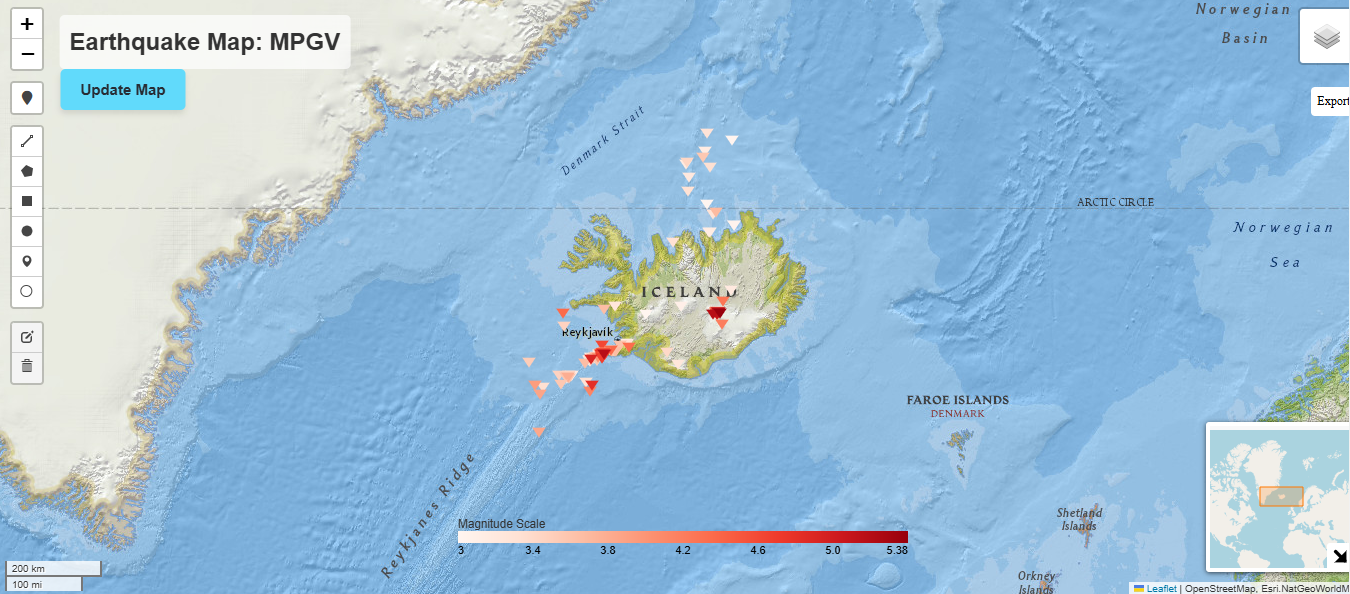
\includegraphics[width=\linewidth, height=7cm]{Screenshots/Folium_Map_version.png}
    \caption{Folium Based Map Version}
\end{figure}

To address these limitations, the project transitioned to a more modernized architecture, combining Flask for backend API services with Vite and React for the frontend. This shift enabled greater interactivity, improved responsiveness, and better scalability by offloading much of the visualization logic to the client side. The new architecture also made it practical to add features like the time slider and the earthquake magnitude scale that would have been awkward to implement in the earlier server-rendered approach.

Python remains the core language of the backend due to its mature ecosystem for web development and data processing. Flask serves as the lightweight web framework responsible for handling API requests and serving earthquake data in JSON format. The data ingestion logic combines traditional HTML scraping from the Icelandic Meteorological Office’s MPGV archive (\texttt{hraun.vedur.is}) with high-frequency seismic data fetched through the Skjálftalísa API. MPGV records are collected using \texttt{BeautifulSoup} and \texttt{requests}, while Skjálftalísa events are retrieved in structured JSON form and stored in a dedicated raw-data table. Both sources are cleaned, normalised, and written to an SQLite database. A reconciliation algorithm subsequently merges MPGV and Skjálftalísa events into a unified catalogue based on temporal, spatial, and magnitude-based matching rules.
The result is a clean, queryable catalogue with no duplicated entries.

Unlike the earlier implementation, where filtering and processing were performed on the backend and visualised through static Folium maps, the new system uses React to dynamically display earthquake data on an interactive map. An intermediate version of the frontend used the Google Maps JavaScript API for geospatial rendering; however, this introduced a dependency on a paid API key and vendor-specific billing. The current version replaces Google Maps with Leaflet, an open-source mapping library, integrated through \texttt{react-leaflet}. This design lets the frontend render maps using freely available tile services and update in place without full page reloads or external API credentials, something that was difficult to achieve in the earlier backend-heavy architecture.

Vite, a modern build tool and development server, was chosen for the frontend instead of the traditional Create React App. Vite accelerates development through faster builds, hot module replacement, and optimized performance. With React’s component-based structure, the frontend is modular and scalable, making it easier to introduce new features. Dependencies for the backend are managed through a \texttt{requirements.txt} file, including Flask, pandas, requests, BeautifulSoup, SQLAlchemy for database management, APScheduler for automated updates, and additional modules for Skjálftalísa ingestion, EPOS ShakeMap verification, and volcano data retrieval.
On the frontend, dependencies are tracked in \texttt{package.json}, including React~18, \texttt{react-leaflet}~4.2 and \texttt{leaflet}~1.9 for map rendering, \texttt{leaflet.heat} for heatmap visualization, \texttt{axios} for HTTP communication, and \texttt{lodash} for utility functions. The previous version used \texttt{@react-google-maps/api} for Google Maps integration; this dependency has been entirely removed in the current Leaflet-based architecture.

\begin{figure}[H]
    \centering    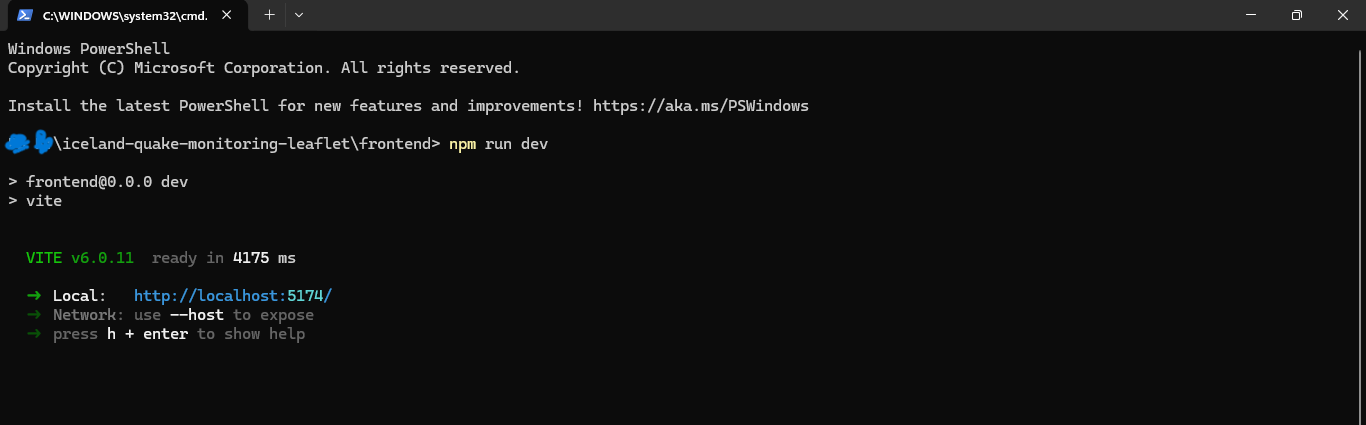
\includegraphics[width=\linewidth, height=7cm]{Screenshots/Vite_terminal.png}
    \caption{Vite development server successfully started for the React frontend, running at \texttt{http://localhost:5174/} locally.}
\end{figure}

The move to a Vite + React frontend and a lightweight Flask API backend resolved the main limitations of the earlier version, page reloads on every interaction, tight coupling between scraping and rendering, and slow startup, while keeping the overall architecture simple enough to extend later.

\newpage

\subsection{Data Sources}
The \textbf{MPGV Monitor} system integrates multiple authoritative datasets to construct a unified and reliable earthquake catalogue for Iceland. In earlier versions of the project, the only data source was the Icelandic Meteorological Office’s HTML-based MPGV archive (\href{http://hraun.vedur.is/ja/Mpgv/}{hraun.vedur.is}), which contains monthly tables of date-time, location, depth, and magnitude values. Although the structure of the MPGV pages is predictable and suitable for automated scraping, relying solely on this source limited temporal resolution and restricted the system’s ability to incorporate higher-frequency seismic data.

\vspace{8\baselineskip}


\begin{figure}[H]

    \centering    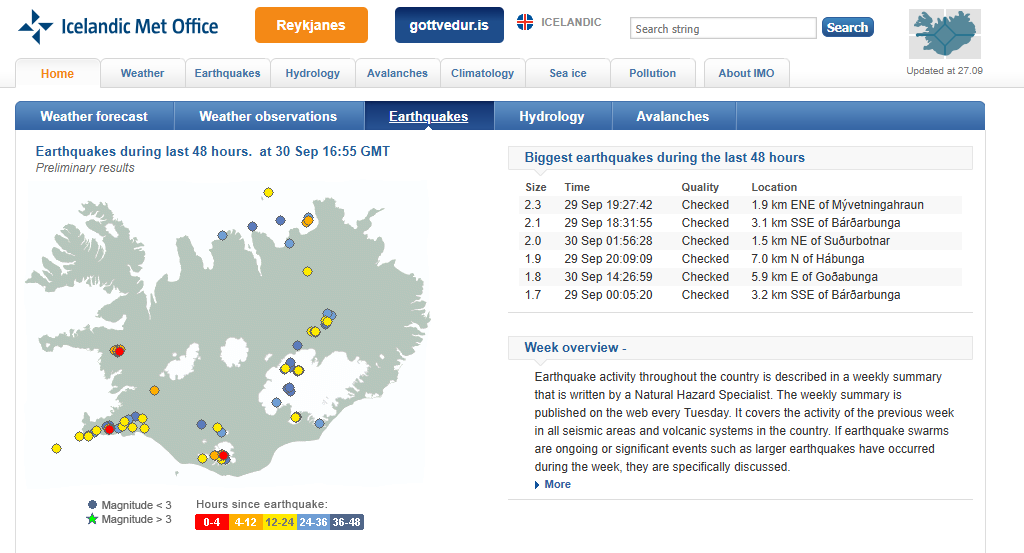
\includegraphics[width=\linewidth, height=8cm]{Screenshots/hraun_vedur.png}

    \caption{Icelandic Meteorological Office website (\texttt{vedur.is}).}

\end{figure}

\begin{figure}[H]

    \centering

    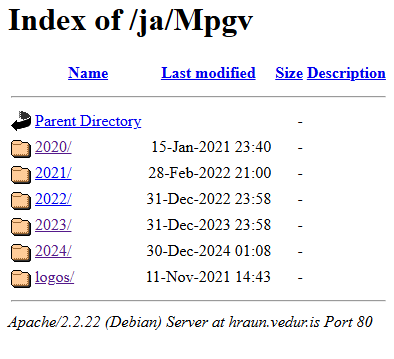
\includegraphics[width=0.45\textwidth, height=7cm]{Screenshots/Year.png}

    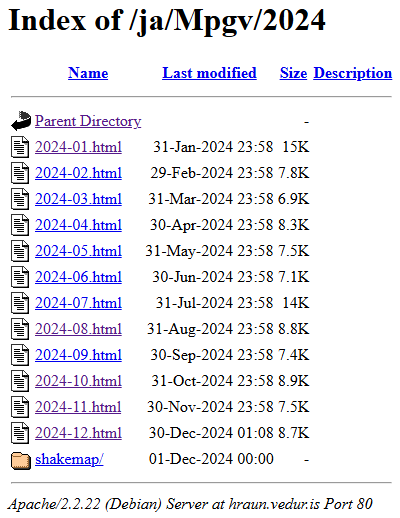
\includegraphics[width=0.45\textwidth, height=8cm]{Screenshots/Month.png}

    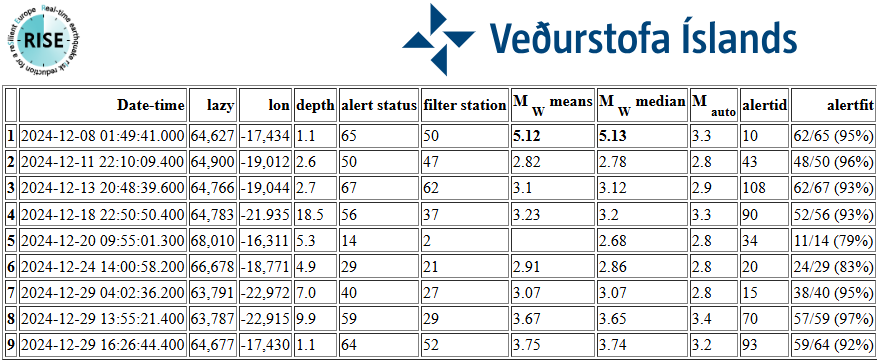
\includegraphics[width=\linewidth]{Screenshots/Data.png}

    \caption{Examples of year-based, month-based, and tabular earthquake data sources from Mpgv (\texttt{hraun.vedur.is})}

\end{figure}

\newpage


To address these limitations, the current architecture combines MPGV records with data from the \textbf{Skjálftalísa API}, a machine-readable web service maintained by the Icelandic Meteorological Office that provides earthquake information in JSON format. Skjálftalísa delivers higher temporal precision, richer metadata, and unique event identifiers, enabling more accurate and complete cataloguing of seismic activity. Events retrieved from Skjálftalísa are stored in a dedicated raw-data table, while MPGV events are stored separately to preserve their original structure.

\begin{figure}[H]

    \centering    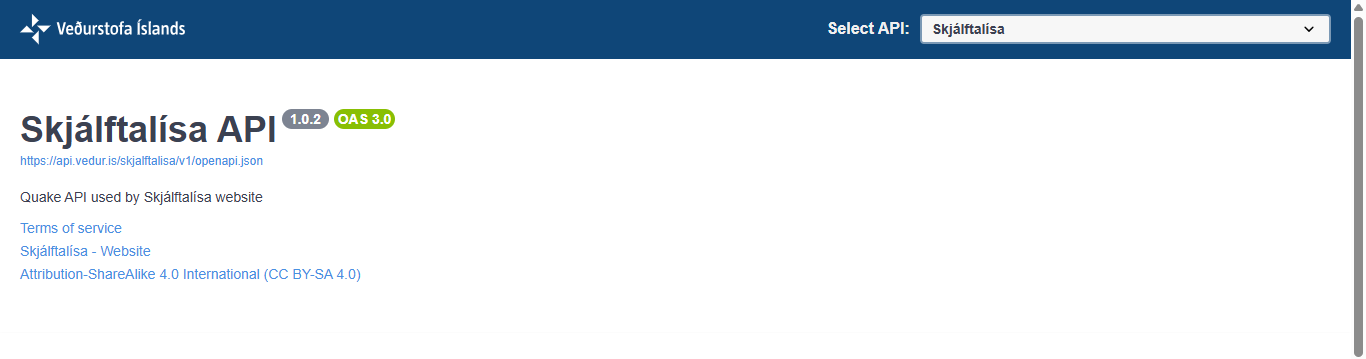
\includegraphics[width=\linewidth, height=6cm]{Screenshots/S_Api.png}

    \caption{Official Skjálftalísa API documentation provided by the Icelandic Meteorological Office, showing the REST interface used to retrieve machine-readable earthquake data.}

\end{figure}

\begin{figure}[H]

    \centering    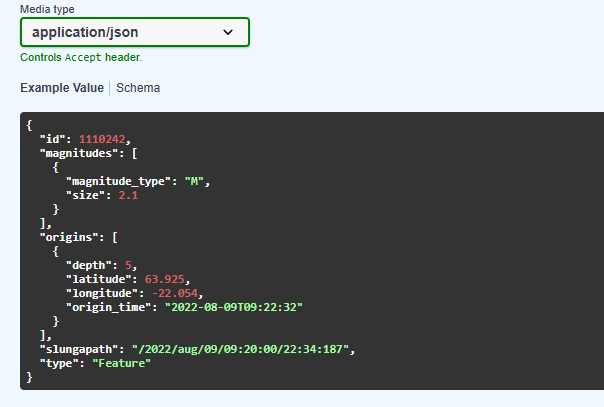
\includegraphics[width=\linewidth, height=10cm]{Screenshots/Quake_event.png}

    \caption{Example of a Skjálftalísa API JSON response, illustrating the structure of event metadata including magnitude, depth, coordinates, and origin time.}

\end{figure}

A reconciliation algorithm subsequently merges MPGV and Skjálftalísa events into a unified dataset. This process compares events from both sources using temporal proximity, spatial distance, and magnitude similarity to identify matches and resolve duplicates. The resulting merged catalogue, stored in the \texttt{earthquake\_merged} table, provides improved accuracy in event location, depth, and magnitude while ensuring consistency across updates.

In addition to earthquake data, the system ingests auxiliary information from the \textbf{EPOS Iceland} APIs. The EPOS Volcanoes API supplies volcano locations, elevation values, and descriptive metadata, enabling the display of volcano overlays on the map. The EPOS ShakeMap API provides shaking intensity products that can be associated with individual earthquakes; these are cross-referenced against the merged catalogue to supply optional ShakeMap links for supported events. This extra data lets users see which volcanoes are near a cluster and check whether EPOS has a ShakeMap for a given event.

All data from MPGV, Skjálftalísa, and EPOS endpoints are stored in an SQLite database, which supports efficient queries, automated updates, and consistent long-term storage. The backend exposes this information through Flask API routes, while the frontend retrieves and visualizes the data in real time on a Leaflet-based map using free tile providers (OpenStreetMap, Esri World Imagery, and CartoDB Dark Matter). Features such as the time slider, magnitude scale, timeline-based or magnitude-based marker colouring, density heatmap visualization, volcano overlays, and ShakeMap integration are made possible by this multi-source ingestion framework.

Taken together, the MPGV scraper, Skjálftalísa client, EPOS integration, and reconciliation pipeline give the system a single, deduplicated catalogue drawn from multiple independent sources. This catalogue underpins every frontend feature, from time-filtered marker rendering to ShakeMap drill-down, and can accommodate new feeds without restructuring the existing pipeline.

\newpage

% ============================ CHAPTER 4 ============================

\section{Data Scraping and Merging}

The \textbf{MPGV Monitor} system relies on a unified earthquake catalogue that combines multiple sources into a single, quality-controlled dataset. This chapter traces the evolution of the data pipeline from an initial single-month prototype to the current multi-source ingestion workflow and introduces the conceptual design of the reconciliation process. The emphasis is on \emph{how} the scraping and merging strategy matured over time, rather than on the implementation details of the backend, which are discussed separately in Chapter~5.

\vspace{0.4cm}

\subsection{Initial Approach}

The earliest implementation of data scraping focused on extracting earthquake records for a single month, October~2023, from the Icelandic Meteorological Office’s MPGV archive. This preliminary test served as a proof of concept, demonstrating that the monthly HTML pages on \texttt{hraun.vedur.is} could be parsed reliably and that automated harvesting of Icelandic earthquake data was technically feasible.

Using Python libraries such as \texttt{requests}, \texttt{BeautifulSoup}, and \texttt{pandas}, the script retrieved and parsed the HTML table, cleaned the dataset, and retained only records with magnitudes $\geq 3.0$. The processed data was then stored in a text file for basic visualization and preliminary validation.

\begin{figure}[H]
\centering
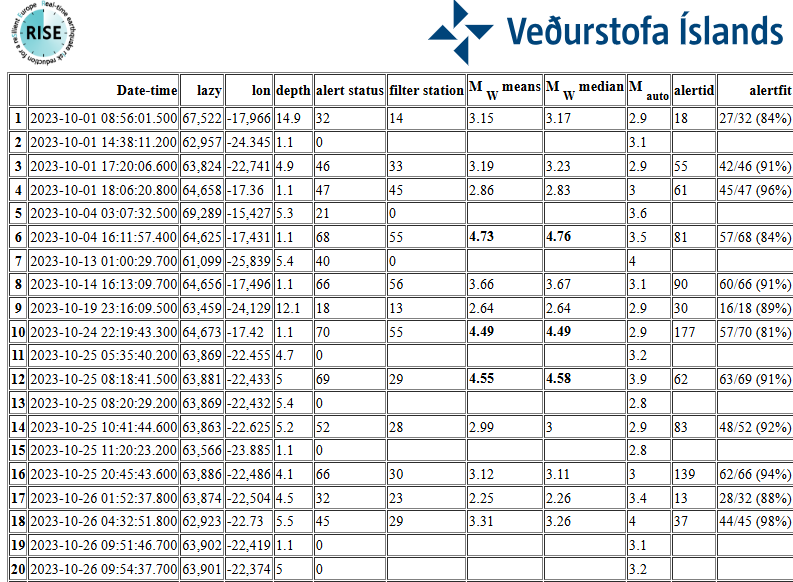
\includegraphics[width=\linewidth]{Screenshots/Raw_Data.png}
\caption{Extract from the initial raw MPGV dataset for October 2023 after basic cleaning and magnitude filtering.}
\end{figure}

The initial dataset contained 30 entries, which were reduced to 15 after filtering. Although limited in scope, this experiment confirmed that automated scraping was viable, that the MPGV HTML tables were sufficiently stable for programmatic parsing, and that the extracted attributes (date--time, latitude, longitude, depth, magnitude) could be normalized for further processing.

This first prototype treated the MPGV archive as a static data source and did not attempt to maintain a historical catalogue or support continuous updates. Nevertheless, it provided a concrete starting point for designing a more general data pipeline.

\vspace{0.4cm}

\subsection{Previous Approaches}

As the project evolved, two intermediate approaches were developed before arriving at the final database-driven, multi-source system. Both of these methods still relied on MPGV as the sole data provider, but they gradually expanded the temporal coverage and improved the structure of the stored data.

\subsubsection*{Manual Scraping with Text File Storage}

In the first extension, the scraper was generalised to fetch not only October~2023 but also the most recent month’s dataset from MPGV and store it locally in a plain-text file. Data was updated only when the script was executed manually. This approach was sufficient for exploratory analysis and basic visualisations, since the text file could be reloaded into Python notebooks or plotting tools.

However, the method had three important limitations. First, it could not efficiently retrieve historical records spanning multiple years. Second, each manual run overwrote the previous file, making it difficult to preserve a consistent long-term catalogue. Third, the loosely structured text format complicated downstream processing and increased the risk of format inconsistencies.

\subsubsection*{Dynamic Scraping with CSV Storage}

To expand coverage and improve structure, the scraper was redesigned to traverse multiple years and months programmatically, consolidating results into a single CSV file. Instead of targeting one fixed month, the script discovered available year and month links from the MPGV index page and iterated over them to harvest all records since June~2020.

\textbf{Code Snippet: Aggregating Monthly Records into CSV}

\begin{verbatim}
def scrape_all_to_csv():
    all_data = pd.DataFrame(columns=['DateTime','Lat','Lon','Depth','Mw'])
    response = requests.get(BASE_URL)
    soup = BeautifulSoup(response.content, 'html.parser')

    year_links = [a['href'].strip('/') for a in soup.find_all('a')
                  if a['href'].endswith('/')]

    for year in year_links:
        for month in get_months(year):
            monthly_data = get_monthly_data(year, month)
            all_data = pd.concat([all_data, monthly_data])

    all_data.to_csv("earthquakes.csv", index=False)
\end{verbatim}

This CSV-based approach addressed some of the shortcomings of the manual text-file workflow. It allowed the entire MPGV archive to be downloaded in a reproducible manner, enabled simple filtering and aggregation using \texttt{pandas}, and provided a convenient input format for early visualisation experiments.

On the other hand, several issues emerged as the dataset grew. Maintaining synchronisation between the CSV file and any downstream visualisation or web frontend became increasingly fragile: every update required regenerating and redistributing the entire file. Moreover, performing repeated full-archive scrapes was inefficient and unnecessary once most historical data had already been ingested. These drawbacks motivated a transition from flat-file storage to a dedicated database.

\newpage

\textbf{Flowchart of CSV-Based Approach}

\vspace{0.7cm}

\begin{figure}[H]

\centering    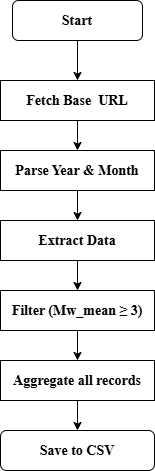
\includegraphics[width=0.3\textwidth, height=12cm]{Screenshots/CSV-based solution.png}

\end{figure}

The CSV-based solution therefore formed an important intermediate step: it demonstrated that the full MPGV archive could be harvested automatically and analysed as a coherent dataset, while highlighting the need for a database-backed backend that could handle concurrent access and automated updates.

\vspace{0.4cm}

\subsection{Current Approach: Multi-Source Ingestion and Conceptual Merging}

The final design replaces the earlier MPGV-only, file-based workflow with an integrated, multi-source ingestion pipeline backed by an SQLite database. Instead of treating MPGV as the sole data provider, the system now combines three authoritative sources:

\begin{itemize}
    \item the MPGV HTML archive (curated earthquake solutions),
    \item the Skjálftalísa JSON API (high-frequency preliminary detections),
    \item and EPOS Iceland endpoints for volcano and ShakeMap metadata.
\end{itemize}

All data is written to \texttt{earthquakes.db}, where it is organised into separate tables for MPGV events, Skjálftalísa raw detections, a merged catalogue, and auxiliary volcano and ShakeMap information. This chapter focuses on the \emph{data-level} view of this pipeline; the concrete SQLAlchemy models, scheduler configuration, and Flask routes are described in detail in Chapter~5.

\subsubsection*{Automated Updates with Periodic Jobs}

In the current system, updates are no longer triggered manually. Instead, a periodic job executes the ingestion and merging pipeline at fixed intervals. Conceptually, each cycle performs three main operations:

\begin{enumerate}
    \item Scrape the latest MPGV records and append any new events to the MPGV table.
    \item Fetch recent Skjálftalísa detections and update the raw Skjálftalísa table.
    \item Run the reconciliation algorithm to produce an up-to-date unified catalogue.
\end{enumerate}

Only events with magnitude $\geq 2.7$ are retained. Duplicate entries are avoided by combining database-level uniqueness constraints (for example on timestamp and coordinates) with event matching rules based on temporal proximity, spatial distance, and magnitude similarity. The effect is that repeated runs of the pipeline are \emph{idempotent}: if no new earthquakes have occurred, the contents of the merged catalogue remain unchanged, even though the reconciliation logic is executed again.

\subsubsection*{Conceptual Ingestion and Merge Pipeline}

From a conceptual perspective, the multi-source pipeline can be expressed as a three-stage dataflow:

\begin{enumerate}
    \item \textbf{Ingestion}: each source-specific module (MPGV scraper, Skjálftalísa client, EPOS volcano loader) harvests data from its respective endpoint and writes normalised records into dedicated tables.
    \item \textbf{Reconciliation}: a matching algorithm compares candidate events from MPGV and Skjálftalísa and decides whether they refer to the same earthquake based on time, distance, and magnitude tolerances.
    \item \textbf{Merged catalogue}: for each MPGV event, the algorithm either finds a corresponding Skjálftalísa detection and records a \texttt{matched} entry or classifies it as \texttt{v\_only} if no suitable counterpart exists. The result is stored in a unified table that is consumed by the frontend.
\end{enumerate}

At this stage, it is useful to view reconciliation primarily as a \emph{data integration} problem: two different catalogues with slightly different coverage and timing must be aligned into a single, provenance-aware representation. The exact mathematical thresholds, depth-selection policies, and implementation details of the matching algorithm are presented in Chapter~5, where the reconciliation logic is discussed as part of the backend architecture.

\subsubsection*{Illustrative Ingestion and Merging Workflow}

The overall workflow of the current pipeline can be summarised as a recurring multi-source process that culminates in a single display catalogue:

\vspace{0.7cm}

\begin{figure}[H]

\centering    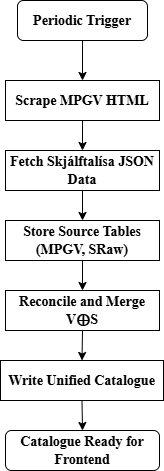
\includegraphics[width=0.3\textwidth, height=12cm]{Screenshots/Data_pipeline.png}

\end{figure}

In the deployed system, the unified catalogue is exposed to the React frontend through RESTful API endpoints and rendered on an interactive Leaflet-based map. The design choice to separate ingestion, reconciliation, and delivery into distinct stages makes it easier to evolve each component independently. For example, additional data sources or alternative matching strategies can be incorporated without changing the general flow from raw source tables to a merged, visualisation-ready dataset. Similarly, the recent migration of the frontend rendering layer from Google Maps to Leaflet required no modifications to the data pipeline or API contracts.

\subsubsection*{Evolution of the Data Pipeline}

Overall, the data pipeline for \textbf{MPGV Monitor} has progressed through three major stages. The initial prototype scraped a single month of MPGV data into text files, suitable only for small-scale experiments. The subsequent CSV-based approach introduced dynamic scraping across years and months, enabling historical analysis but still relying on manual updates and monolithic flat-file storage. The final pipeline adopts a database-centric, multi-source architecture with automated updates and a dedicated reconciliation step that integrates MPGV and Skjálftalísa catalogues.

Each stage fixed a concrete problem left by the one before it. Text files broke under concurrent access. CSVs handled one source well enough but fell apart when a second catalogue had to be merged in. Only after moving to a database-backed pipeline could the system run continuous, unattended updates, which is the minimum bar for anything calling itself a real-time monitor. The next chapter describes the backend that grew out of this final stage: its database schema, scheduling infrastructure, reconciliation algorithm, ShakeMap validation pipeline, and the Flask API layer that hands the merged catalogue to the frontend.

% ============================ CHAPTER 5 ============================

\section{Backend Development}

The backend of the \textbf{MPGV Monitor} system is implemented as a persistent Flask application that orchestrates data ingestion, reconciliation, storage, and delivery to the frontend. In contrast to the early prototypes described in Chapter~3, where scraping logic was embedded in standalone scripts and results were stored in flat files, the current backend adopts a modular architecture built around SQLAlchemy ORM models, an SQLite database, a periodic scheduling subsystem, and a set of RESTful API endpoints.

At a high level, the backend operates through several interconnected layers, illustrated in Figure~\ref{fig:system-architecture}. Source-specific ingestion modules collect information from MPGV, Skjálftalísa, and EPOS endpoints; a reconciliation layer matches and merges events from the two seismic catalogues; a validation layer associates EPOS ShakeMaps with merged events; and the resulting products are stored in an SQLite database and exposed to the React frontend through a JSON-based API. These components run continuously under the coordination of \texttt{APScheduler}, which triggers the automated update cycle every three minutes and keeps the local catalogue synchronized with the external services.

\vspace{0.7cm}

\begin{figure}[H]

\centering    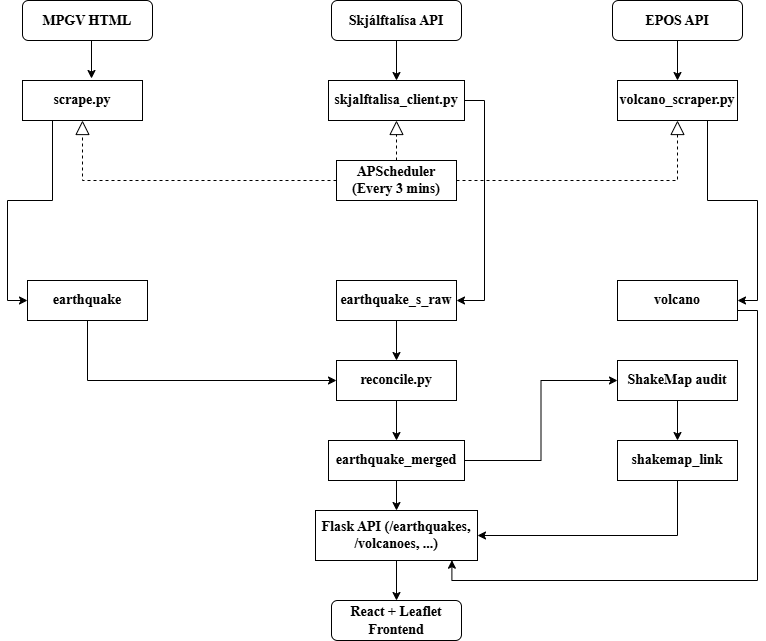
\includegraphics[width=\linewidth, height=12cm]{Screenshots/MPGV_sys_arc.png}

\caption{Full system architecture of MPGV Monitor, showing external data sources, ingestion modules, database tables, reconciliation pipeline, API layer, and frontend.}

\end{figure}

\subsection{Core Database Models}

A central element of the backend architecture is the structured SQLite schema, exposed through SQLAlchemy ORM classes in the Flask application. The schema deliberately separates raw source tables from the derived, unified catalogue and auxiliary products. This separation provides consistency, traceability, and efficient querying across the entire pipeline. The main tables are \texttt{Earthquake} for MPGV-sourced events, \texttt{EarthquakeSRaw} for Skjálftalísa detections, \texttt{EarthquakeMerged} for the unified view, \texttt{Volcano} for EPOS volcano metadata, and \texttt{ShakeMapLink} for cached ShakeMap validation results.

The \textbf{Earthquake} model represents earthquake events scraped from the MPGV HTML archive (denoted internally as \emph{v} events). MPGV entries are curated and validated by the Icelandic Meteorological Office and therefore act as the authoritative baseline for the system. The table stores attributes such as timestamp, location, depth, and magnitude, all normalised from the monthly pages on \texttt{hraun.vedur.is}. A uniqueness constraint on the combination of timestamp and coordinates prevents duplicate insertions during repeated ingestion runs.

\begin{verbatim}
class Earthquake(db.Model):
    id         = db.Column(db.Integer, primary_key=True)
    date_time  = db.Column(db.String, index=True, nullable=False)
    latitude   = db.Column(db.Float, nullable=False)
    longitude  = db.Column(db.Float, nullable=False)
    depth      = db.Column(db.Float, nullable=False)
    mw_mean    = db.Column(db.Float, nullable=False)
\end{verbatim}

The \textbf{EarthquakeSRaw} model stores raw Skjálftalísa API detections (denoted as \emph{s} events). Skjálftalísa provides high-frequency, preliminary seismic detections that often appear before the corresponding MPGV solutions. These records are stored with their original event identifiers, magnitudes, timestamps, and coordinates. Because Skjálftalísa can include small or transient events and early solutions, the raw table deliberately preserves the data as-ingested to maintain provenance for the reconciliation step.

\begin{verbatim}
class EarthquakeSRaw(db.Model):
    id         = db.Column(db.Integer, primary_key=True)
    event_id   = db.Column(db.String, unique=True, nullable=False)
    date_time  = db.Column(db.String, index=True, nullable=False)
    latitude   = db.Column(db.Float, nullable=False)
    longitude  = db.Column(db.Float, nullable=False)
    depth      = db.Column(db.Float)
    magnitude  = db.Column(db.Float)
\end{verbatim}

The \textbf{EarthquakeMerged} model represents the unified catalogue that is served directly to the frontend. Each row corresponds to a single earthquake that has either been matched across MPGV and Skjálftalísa or originates from only one of them. During reconciliation, the system compares events from both sources using temporal, spatial, and magnitude thresholds (see Section~\ref{subsec:reconcile}) and decides whether they describe the same physical event. If so, the merged entry inherits MPGV parameters while retaining the Skjálftalísa identifier and diagnostic metrics such as time and distance offsets. Otherwise, the event is recorded as MPGV-only.

\begin{verbatim}
class EarthquakeMerged(db.Model):
    id           = db.Column(db.Integer, primary_key=True)
    date_time    = db.Column(db.String, index=True, nullable=False)
    latitude     = db.Column(db.Float, nullable=False)
    longitude    = db.Column(db.Float, nullable=False)
    depth        = db.Column(db.Float)
    mw_mean      = db.Column(db.Float, nullable=False)

    status       = db.Column(db.String, nullable=False)   # 'matched' | 'v_only'
    v_src_key    = db.Column(db.String)
    s_event_id   = db.Column(db.String)
    match_dt_sec = db.Column(db.Float)
    match_dist_km= db.Column(db.Float)
    match_dm     = db.Column(db.Float)
\end{verbatim}

The \textbf{Volcano} table stores metadata for Icelandic volcanoes obtained from EPOS Iceland, including their geographic locations and elevations. This information is used to draw volcano overlays in the frontend and to support contextual analyses such as distance-to-volcano queries or swarm clustering.

\begin{verbatim}
class Volcano(db.Model):
    id           = db.Column(db.Integer, primary_key=True)
    name         = db.Column(db.String, nullable=False)
    description  = db.Column(db.Text)
    elevation_m  = db.Column(db.Float)
    elevation_ft = db.Column(db.Float)
    latitude     = db.Column(db.Float, nullable=False)
    longitude    = db.Column(db.Float, nullable=False)
    last_eruption= db.Column(db.String)
\end{verbatim}

Finally, the \textbf{ShakeMapLink} table acts as a cache of EPOS ShakeMap products associated with catalogued events. For each event timestamp, it stores the URL of the chosen ShakeMap, together with metadata describing the matching quality (time difference, spatial distance, and magnitude difference between the event and the ShakeMap solution).

\begin{verbatim}
class ShakeMapLink(db.Model):
    __tablename__ = "shakemap_links"

    dt          = db.Column(db.String, primary_key=True)
    url_view_file = db.Column(db.String)
    origin_time = db.Column(db.String)

    sm_lat   = db.Column(db.Float)
    sm_lon   = db.Column(db.Float)
    sm_mag   = db.Column(db.Float)
    sm_depth = db.Column(db.Float)

    dt_sec   = db.Column(db.Float)
    dist_km  = db.Column(db.Float)
    dm       = db.Column(db.Float)

    status   = db.Column(db.String)  # "valid" | "no_candidate" | "no_valid" | "error"
    note     = db.Column(db.String)
\end{verbatim}

The raw source tables are never overwritten or merged in place; they stay intact so that any reconciliation run can be repeated or audited. The merged catalogue, volcano metadata, and ShakeMap links are all derived products that can be rebuilt from the raw tables if the matching rules change.

\subsection{Dynamic Data Ingestion}

The dynamic ingestion pipeline is responsible for keeping the local database synchronized with the external MPGV, Skjálftalísa, and EPOS services. Rather than relying on manual runs or static files, the system uses three dedicated modules, \texttt{scrape.py}, \texttt{skjalftalisa\_client.py}, and \texttt{volcano\_scraper.py}, to harvest and normalise data from each source. All ingestion operations write directly into the ORM-backed tables described above.

A few practical realities shaped how the ingestion works. The external services go down from time to time, and occasionally return malformed responses, so each module has to fail without leaving the local database in a half-written state. Updates need to happen often enough that the map feels live, but not so often that the third-party APIs start rejecting requests. Raw records stay in their own tables so the merging step can be re-run on its own if the algorithm changes. And if a new data source appears later, plugging it in should not mean rewriting the existing modules. In practice, each ingestion module wraps its own networking, error handling, and field normalisation behind a single callable that the scheduler fires every three minutes.

\paragraph{MPGV Scraper.}

The MPGV scraper, implemented in \texttt{scrape.py}, parses the monthly HTML pages published by the Icelandic Meteorological Office. For each month, the scraper retrieves the \texttt{<table>} element containing earthquake records, converts its rows into Python dictionaries, cleans and normalises the values, and applies a magnitude threshold so that only events with $Mw_{\text{mean}} \geq 2.7$ are retained. Records with missing or malformed coordinates, depth, or magnitude are discarded to avoid polluting the catalogue with incomplete entries. A uniqueness constraint on \texttt{(date\_time, latitude, longitude)} prevents duplicate rows when the scraper is re-run.

\paragraph{Skjálftalísa Client.}

The Skjálftalísa ingestion module, implemented in \texttt{skjalftalisa\_client.py}, interacts with the JSON-based Skjálftalísa API. The service returns column-oriented arrays of values, which the client converts into row-wise dictionaries containing event IDs, timestamps, latitudes, longitudes, depths, and magnitudes. Timestamps are normalised to the uniform format \texttt{YYYY-MM-DD HH:MM:SS} in UTC, and magnitudes are converted to floating-point values with appropriate filtering. The resulting records are inserted into the \texttt{earthquake\_s\_raw} table, keyed by Skjálftalísa’s \texttt{event\_id} for later matching.

\paragraph{EPOS Volcano Scraper.}

The \texttt{volcano\_scraper.py} module fetches volcano metadata from the EPOS Iceland API. Because EPOS exposes several endpoints and data formats, the scraper performs additional normalisation to reconcile different field names (for example, \texttt{lat\_dd} versus \texttt{latitude}) and ensure that all entries are represented in a consistent schema. Elevation is stored in metres and also converted to feet for convenience. This process populates the \texttt{volcano} table with up-to-date volcano locations and basic descriptive information.

\paragraph{Operational Characteristics.}

To prevent transient issues from corrupting the database, each ingestion module handles network timeouts, retries, and schema changes defensively. Failed cycles do not overwrite existing data, and exceptions are logged for later inspection. In practice, the ingestion pipeline is also optimised for efficiency: the MPGV scraper re-checks all available months but only inserts genuinely new records thanks to the uniqueness constraint, the Skjálftalísa client typically fetches only the last \emph{n} days of activity, and EPOS metadata is refreshed infrequently, since volcano properties evolve slowly on the timescale of the deployment.

\paragraph{Dataset Composition.}

After a full historical ingestion from June~2020 onwards, the three most relevant tables contain the following counts:

\begin{table}[H]
\centering
\begin{tabular}{l r}
\hline
\textbf{Dataset} & \textbf{Number of Events} \\
\hline
MPGV source table (\texttt{earthquake})                    & 1781 \\
Skjálftalísa raw table (\texttt{earthquake\_s\_raw})       & 4906 \\
Merged table (\texttt{earthquake\_merged})                 & 1781 \\
\quad \textit{Matched events} (\texttt{status = 'matched'})   & 1447 \\
\quad \textit{MPGV-only events} (\texttt{status = 'v\_only'}) & 334  \\
\hline
Coverage (\% matched in merged table)                      & 81.2\% \\
\hline
\end{tabular}
\caption{Summary of MPGV, Skjálftalísa, and merged earthquake datasets in the MPGV Monitor database.}
\label{tab:data-coverage}
\end{table}

These statistics highlight the complementary value of Skjálftalísa: more than 80\,\% of MPGV events have a corresponding Skjálftalísa detection, which both validates the matching strategy and confirms the consistency of the two catalogues. The remaining 19\,\% of MPGV events labelled as \texttt{v\_only} either fall outside Skjálftalísa’s temporal window or correspond to events that the API does not report.

\subsection{Automated Scheduling}

Automated ingestion in \textbf{MPGV Monitor} is driven by \texttt{APScheduler}, which periodically triggers a composite backend job without any manual intervention. The scheduler is configured in \texttt{app.py} and attached to the Flask application context. It registers a recurring job that executes the entire ingestion and merging workflow at a fixed interval:

\begin{verbatim}
scheduler.add_job(
    scheduled_scrape,
    "interval",
    minutes=3,
    max_instances=1
)
\end{verbatim}

The choice of a three-minute interval reflects a compromise between data freshness and resource usage. Skjálftalísa can update at sub-minute cadence, whereas MPGV solutions are published on scales of tens of minutes to hours. Running the full update every three minutes ensures that Skjálftalísa detections are incorporated soon after they are available, while also catching new MPGV entries in a timely fashion, without placing excessive load on the external services or the local SQLite database.

The \texttt{max\_instances=1} parameter is critical from a reliability perspective. It guarantees that a new scheduler run is not started while the previous one is still active, thereby avoiding overlapping writes and potential race conditions. Each scheduled execution of \texttt{scheduled\_scrape} performs a full pass of the pipeline: MPGV scraping, Skjálftalísa fetching, reconciliation into the merged table, and optional ShakeMap validation.

In the current deployment, where the entire historical catalogue from June~2020 has already been ingested, many scheduler cycles log messages such as \enquote{\texttt{:)\ 0 new earthquake records added to SQLite via Flask.}} followed by \enquote{\texttt{Merged rows written:1753}}. This behaviour illustrates that the pipeline is idempotent: the job can be re-run safely even when no new events are available, and the content of the merged table remains stable. When new earthquakes are published by the Icelandic Meteorological Office, the same mechanism automatically incorporates them into both the MPGV table and the unified catalogue.

From an architectural viewpoint, the scheduler runs as a background component alongside the Flask application. HTTP endpoints such as \texttt{/earthquakes}, \texttt{/volcanoes}, and \texttt{/shakemap/\{dt\}} remain responsive while ingestion is in progress. Because the ingestion and reconciliation steps operate within database transactions, partial failures (for example, a temporary API outage) do not corrupt existing tables: exceptions are caught and logged, and the next scheduled cycle resumes from a clean state.

\vspace{0.7cm}

\begin{figure}[H]

\centering    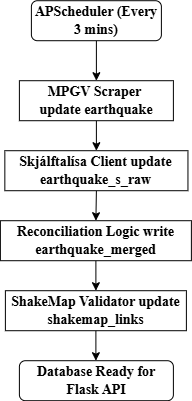
\includegraphics[width=0.3\textwidth, height=10cm]{Screenshots/APScheduler_working.png}
\caption{Automated scheduling workflow coordinating ingestion, reconciliation, and ShakeMap validation.}
\end{figure}

\newpage

\subsection{Reconciliation and Merging}
\label{subsec:reconcile}

The reconciliation algorithm integrates MPGV (\textit{v}) events with Skjálftalísa (\textit{s}) detections to form a unified earthquake catalogue. Its purpose is to determine whether a pair of events from the two sources represents the same physical earthquake. Matching is based on three criteria: temporal proximity, spatial distance, and similarity in magnitude.

For an MPGV event $v$ and a Skjálftalísa event $s$, a valid match must satisfy:

\[
|\Delta t| \leq 2 \text{ seconds}, \qquad
\Delta d < 10 \text{ km}, \qquad
|\Delta Mw| < 3.0,
\]

where $\Delta t$ is the absolute difference in origin times, $\Delta d$ is the great-circle epicentral distance, and $\Delta Mw$ is the magnitude difference. These thresholds were tuned empirically to maximise correct matches while avoiding spurious associations. Compared to an earlier version of the algorithm that used $|\Delta t| < 3$\,s and $|\Delta Mw| < 2.0$, the current thresholds tighten the temporal window to $\pm 2$\,seconds while relaxing the magnitude tolerance to $|\Delta Mw| < 3.0$, reflecting the observation that magnitude estimates can differ substantially between the two catalogues for the same physical event.

At runtime, the system loads all Skjálftalísa detections into a time-indexed structure, enabling efficient lookup of candidate events whose timestamps differ from the corresponding MPGV event by at most two seconds. The overall reconciliation workflow is illustrated in Figure~\ref{fig:reconcile-workflow}. For each MPGV entry, the algorithm retrieves all Skjálftalísa events satisfying the temporal constraint, computes the spatial separation and magnitude deviation, filters out invalid candidates, and classifies the event as either \texttt{v\_only} or \texttt{matched}. If exactly one candidate passes all three thresholds, it is accepted as the match. If two or more candidates pass, the situation is considered ambiguous and the MPGV event falls back to \texttt{v\_only} status rather than risking a spurious association.

\vspace{0.7cm}

\begin{figure}[H]

\centering    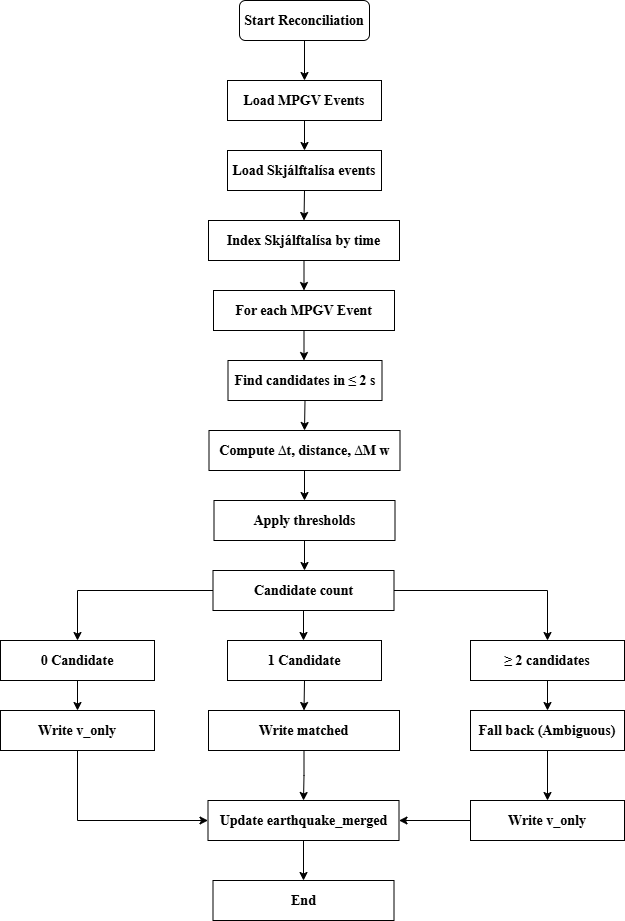
\includegraphics[width=\linewidth, height=20cm]{Screenshots/Reconciliation workflow.png}

\caption{Reconciliation workflow with branching logic and compact layout.}

\end{figure}

The corresponding Python implementation is shown below. It reflects the control flow depicted in Figure~\ref{fig:reconcile-workflow} and implements the threshold rules precisely. Diagnostic information such as time offset (\texttt{match\_dt\_sec}), epicentral distance (\texttt{match\_dist\_km}), and magnitude deviation (\texttt{match\_dm}) is stored alongside each merged event, enabling quality assessment and downstream analysis.

\begin{verbatim}
for v in v_rows:
    candidates = []

    # Search Skjálftalísa events within ±2 seconds of the MPGV timestamp
    for s in s_index.get_window(v.date_time, window_sec=2):
        dt_abs  = abs(v.dt_ts - s.dt_ts)
        dist_km = haversine_km(v.lat, v.lon, s.lat, s.lon)
        dm      = abs(v.mw_mean - (s.magnitude or 0))

        # Candidate must satisfy all three thresholds
        if dt_abs <= 2 and dist_km < 10 and dm < 3.0:
            candidates.append((dist_km, dt_abs, dm, s))

    # No valid Skjálftalísa match → v_only
    if not candidates:
        write_v_only(v)
        continue

    # Exactly one candidate → accept as matched
    # Multiple candidates → ambiguous, fall back to v_only
    if len(candidates) == 1:
        dist, dt_abs, dm, best_s = candidates[0]
        write_matched(v, best_s, dt_abs, dist, dm)
    else:
        write_v_only(v)
\end{verbatim}

Because the reconciliation outcome is recorded in the \texttt{status} field and both MPGV and Skjálftalísa identifiers are kept, every match can be audited after the fact. If the thresholds turn out to be too tight or too loose, the algorithm can be re-tuned and the merge re-run without losing any raw data.

\subsection{ShakeMap Validation Pipeline}
\label{subsec:shakemap}

While the merged earthquake catalogue provides a consistent record of seismicity, it does not directly describe the shaking intensity or ground-motion patterns associated with each event. To enrich the dataset with this information, the system includes a ShakeMap validation pipeline that searches for EPOS Iceland ShakeMap products corresponding to each merged earthquake. The validation logic, implemented in \texttt{shakemap\_validator.py}, queries the EPOS API, evaluates candidate ShakeMaps, and records the most plausible match in the \texttt{shakemap\_links} table.

\subsubsection*{Validation Procedure}

For each event in the merged catalogue with origin time $t$, epicentre $(\phi, \lambda)$, and magnitude $M_w$, the validator performs the following steps:

\begin{enumerate}
    \item \textbf{ShakeMap retrieval.} Query the EPOS ShakeMap API for products occurring within a 30-minute window centred on the event time and lying inside a latitude--longitude bounding box around the event location.
    \item \textbf{Candidate evaluation.} For every returned ShakeMap, compute:
    \[
    |\Delta t| = |t_{\text{event}} - t_{\text{sm}}|, \quad 
    \Delta d = \text{dist}\big((\phi,\lambda), (\phi_{\text{sm}},\lambda_{\text{sm}})\big), \quad
    |\Delta M| = |M_w - M_{w,\text{sm}}|.
    \]
    ShakeMaps exceeding predefined limits on any of these metrics are rejected.
    \item \textbf{Best-match selection.} If multiple valid candidates remain, select the one with the smallest combination of temporal offset, spatial distance, and magnitude deviation using a lexicographic ordering.
    \item \textbf{Database update.} Store the selected ShakeMap (or the failure category) in the \texttt{shakemap\_links} table together with diagnostic values such as \texttt{dt\_sec}, \texttt{dist\_km}, and \texttt{dm}.
\end{enumerate}

If EPOS returns no ShakeMaps for the query window, the event is labelled \texttt{no\_candidate}. If candidates exist but none satisfy the validation thresholds, the status becomes \texttt{no\_valid}. Errors during API retrieval or metadata parsing result in the status \texttt{error}. Recording the failure reason explicitly, rather than silently dropping unmatched events, means the frontend can tell the user \emph{why} no ShakeMap is shown, not just that one is absent.

\vspace{0.7cm}

\begin{figure}[H]

\centering    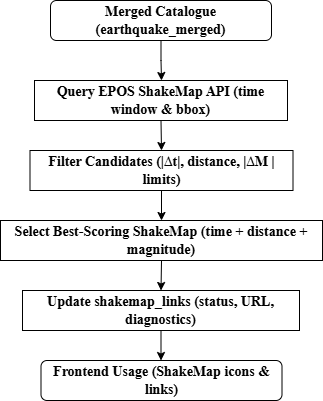
\includegraphics[width=0.4\textwidth, height=8cm]{Screenshots/ShakeMap validation workflow.png}
\caption{ShakeMap validation workflow: retrieving candidates from EPOS, filtering by temporal, spatial, and magnitude thresholds, selecting the best match, and caching results for frontend access.}
\end{figure}

\subsubsection*{Audit Mode and Evaluation Results}

To evaluate the reliability of the matching pipeline and the completeness of EPOS ShakeMap coverage, the script includes an audit mode. Running:

\begin{verbatim}
python shakemap_validator.py
\end{verbatim}

executes the ingestion, reconciliation, and ShakeMap matching workflow for the entire merged catalogue. The script then prints a summary of validation outcomes and writes a CSV report to \texttt{backend/reports/shakemap\_audit.csv}. The audit is particularly useful for monitoring:
\begin{itemize}
    \item how often ShakeMaps exist for Icelandic earthquakes,
    \item how many ShakeMaps are filtered out by the acceptance criteria,
    \item the frequency of EPOS data inconsistencies or retrieval failures,
    \item long-term trends in ShakeMap availability.
\end{itemize}

A representative audit performed on the full catalogue of 1753 merged events produced the distribution shown in Table~\ref{tab:shakemap-audit}. In this run, 465 events successfully matched to a valid ShakeMap, 351 events returned candidates that did not satisfy the threshold criteria, and 937 events resulted in errors due to missing metadata or failed EPOS retrievals. ShakeMap coverage is patchy, only 465 out of 1753 events matched, so the system stores the failure reason rather than silently dropping unmatched events.

\begin{table}[H]
\centering
\begin{tabular}{l r}
\hline
\textbf{ShakeMap Status} & \textbf{Count} \\
\hline
valid          & 465 \\
no\_valid      & 351 \\
error          & 937 \\
\hline
\textbf{Total Events Audited} & 1753 \\
\hline
\end{tabular}
\caption{ShakeMap audit summary produced by running 
\texttt{python shakemap\_validator.py}. 
Events marked \texttt{valid} have an accepted ShakeMap; 
\texttt{no\_valid} events returned ShakeMap candidates that failed the acceptance criteria; 
\texttt{error} indicates failures during API retrieval or metadata parsing.}
\label{tab:shakemap-audit}
\end{table}

\subsection{Flask API Layer}

The final component of the backend is the Flask API layer, which exposes the processed and reconciled data stored in SQLite to the React frontend and external tools such as Postman or command-line clients. All endpoints provide JSON responses, and the API surface is intentionally read-only to preserve database integrity, as ingestion and reconciliation are handled exclusively by the scheduler.

The principal routes implemented in \texttt{app.py} are:

\begin{itemize}
    \item \texttt{/earthquakes} ,  returns the unified catalogue from \texttt{earthquake\_merged}, optionally filtered to the last \emph{N} days via a query parameter. Responses are cached in memory with a 60-second TTL.
    \item \texttt{/earthquakes\_csv} ,  downloads the merged earthquake catalogue as a CSV file, supporting the same optional day-based filtering.
    \item \texttt{/volcanoes} ,  returns volcano metadata from the \texttt{volcano} table for map overlay visualisation.
    \item \texttt{/shakemap\_lookup} ,  queries the EPOS API for ShakeMap data near a specified event (parameters: \texttt{dt}, \texttt{lat}, \texttt{lon}).
    \item \texttt{/shakemap/<dt>} ,  returns a cached or validated ShakeMap link and associated diagnostic metadata for the event whose timestamp is \texttt{<dt>}, if available.
    \item \texttt{/health} ,  returns row counts for the \texttt{earthquake}, \texttt{earthquake\_s\_raw}, and \texttt{earthquake\_merged} tables, useful for operational monitoring.
    \item \texttt{/reconcile} ,  manually triggers a reconciliation run; this endpoint is used exclusively for debugging and evaluation.
    \item \texttt{/scrape-volcanoes} ,  manually triggers a volcano metadata refresh from the EPOS API.
\end{itemize}

A typical endpoint serialises ORM objects into dictionaries and wraps them in a JSON response. For example, the endpoint providing the unified earthquake catalogue is defined as follows:

\begin{verbatim}
@app.route("/earthquakes", methods=["GET"])
def get_earthquake_data():
    with app.app_context():
        rows = EarthquakeMerged.query \
            .order_by(EarthquakeMerged.date_time.desc()) \
            .all()

        return jsonify([
            {
                "Date-time": r.date_time,
                "Latitude":  r.latitude,
                "Longitude": r.longitude,
                "Depth":     r.depth,
                "Mw_mean":   r.mw_mean,
                "status":    r.status
            } for r in rows
        ])
\end{verbatim}

Because the Flask application and the scheduler operate on the same SQLite database, all API calls always return the most up-to-date state of the catalogue without requiring additional scraping at request time. To reduce database load under repeated polling, the \texttt{/earthquakes} endpoint employs an in-memory response cache with a 60-second time-to-live (TTL). The cache is invalidated after each scheduled scrape cycle, ensuring that new data is available to clients within at most one minute of ingestion. Requests that include query parameters (such as \texttt{?days=NN}) bypass the cache to ensure accuracy.

Because reads and writes never compete, the API only reads, the scheduler only writes, user queries stay fast even during an active scrape. The JSON response format is also simple enough that the frontend can render markers, overlays, and ShakeMap icons from lightweight requests. Optional gzip compression via Flask-Compress further reduces response payload sizes for clients that support it.

\subsection{Summary}

In practical terms, the backend does four things: it pulls data from three independent sources, schedules those pulls so nobody has to run them by hand, reconciles the results into one deduplicated catalogue, and hands the catalogue to the frontend through a small set of JSON endpoints. SQLAlchemy wraps every write in a transaction, and each ingestion module keeps its own networking and parsing details private, so when the MPGV page layout changed slightly in late 2025, only \texttt{scrape.py} needed updating.

This turned out to matter more than expected during the Leaflet migration. Because the frontend only ever talks to a few GET endpoints that return filtered JSON, swapping Google Maps for Leaflet did not require a single backend change. The same loose coupling should make it straightforward to add new data sources or richer queries later without reworking the pipeline itself.

\newpage

% ============================ CHAPTER 6 ============================
\section{Frontend Architecture and Implementation}
\label{sec:frontend}

The MPGV Monitor frontend provides the user-facing analytical interface of the system. Its primary responsibility is to transform the reconciled and validated earthquake catalogue produced by the backend into an interactive geospatial environment where users can explore events, apply temporal and magnitude filters, and inspect event-level metadata. The frontend is implemented as a single-page application (SPA) using React~18 with Vite as the build toolchain.

\subsubsection*{Migration from Google Maps to Leaflet}

A previous version of the frontend used the Google Maps JavaScript API for all spatial rendering. While Google Maps provided high-quality cartography and smooth navigation, it introduced several practical constraints: a paid API key was required, usage incurred billing based on map loads, and the proprietary nature of the service created vendor lock-in. These constraints were particularly limiting for a research project intended for eventual handover to the Icelandic Meteorological Office, where ongoing API costs and credential management would add operational burden.

The current version replaces Google Maps entirely with \textbf{Leaflet}~1.9, an open-source JavaScript mapping library, integrated into React via the \texttt{react-leaflet}~4.2 bindings. This migration eliminates the need for any API key, removes usage-based billing, and provides full control over tile sources. The specific tile providers used for each basemap mode are detailed in Section~\ref{subsec:frontend_leaflet}. In addition, the Leaflet-based architecture enabled the introduction of a new heatmap visualization mode, canvas-accelerated marker rendering, and a fully custom zoom-responsive latitude/longitude grid overlay, features that were not present in the Google Maps version.

A key architectural principle of the system is separation of concerns. The backend owns ingestion, reconciliation, ShakeMap validation, and persistence. The frontend consumes curated outputs via explicit API endpoints and performs no reconciliation or validation logic locally. Instead, it focuses on (i) presentation of spatial layers, (ii) interactive filtering and visual encoding, and (iii) contextual inspection of individual events. Keeping these responsibilities apart makes the codebase easier to maintain and guarantees that whatever the map shows comes from the same authoritative catalogue that lives in the database. The best evidence for this separation working as intended is that the entire Google Maps--to--Leaflet migration required zero changes to the backend API or data models.

\subsection{User Interface Overview and Interaction Goals}
\label{subsec:frontend_ui_overview}

The frontend is designed around a map-first workflow. When the web application is opened, the map is displayed immediately in default mode and earthquake markers are rendered without requiring additional user actions. This default behavior supports rapid situational awareness by presenting the full available catalogue at first load.

The interface is composed of a small set of persistent controls arranged around the map canvas:

\begin{itemize}
    \item \textbf{Map menu (top-left):} a hover-activated menu that allows switching between \emph{Map}, \emph{Satellite}, \emph{Dark Mode}, and \emph{Heatmap}. These options provide alternative cartographic contexts while keeping the analytical overlays consistent.
    \item \textbf{Application title (top-center):} fixed title providing clear identity of the system.
    \item \textbf{About button (top-right):} opens a compact modal panel above the map that describes the purpose of MPGV Monitor and its data sources, and provides a CSV data export button.
    \item \textbf{Magnitude scale (right):} a vertical slider for magnitude threshold selection, coupled to a color scale when magnitude-color mode is enabled.
    \item \textbf{TimeWindow slider (left, vertical):} a multi-resolution temporal selector that supports navigating from year-level ranges into month-level and day-level windows. Supports both scroll-wheel zoom and drag-based panning.
    \item \textbf{Color-mode toggle (near the slider controls):} switches marker coloring between timeline-based encoding and magnitude-based encoding. The inactive scale becomes visually muted to reduce ambiguity.
    \item \textbf{Overlay toggles (left side):} switches for showing volcano markers and an optional latitude/longitude grid.
\end{itemize}

The controls work as a coordinated set: time and magnitude act as filters, the color-mode selector changes how the surviving markers are shaded, and the overlay toggles add contextual layers (volcanoes, lat/lon grid) independently of filtering. One deliberate design rule is that changing any filter automatically closes the event-inspection panel, so the user never sees stale detail data that no longer matches the active view.

\begin{figure}[H]
\centering
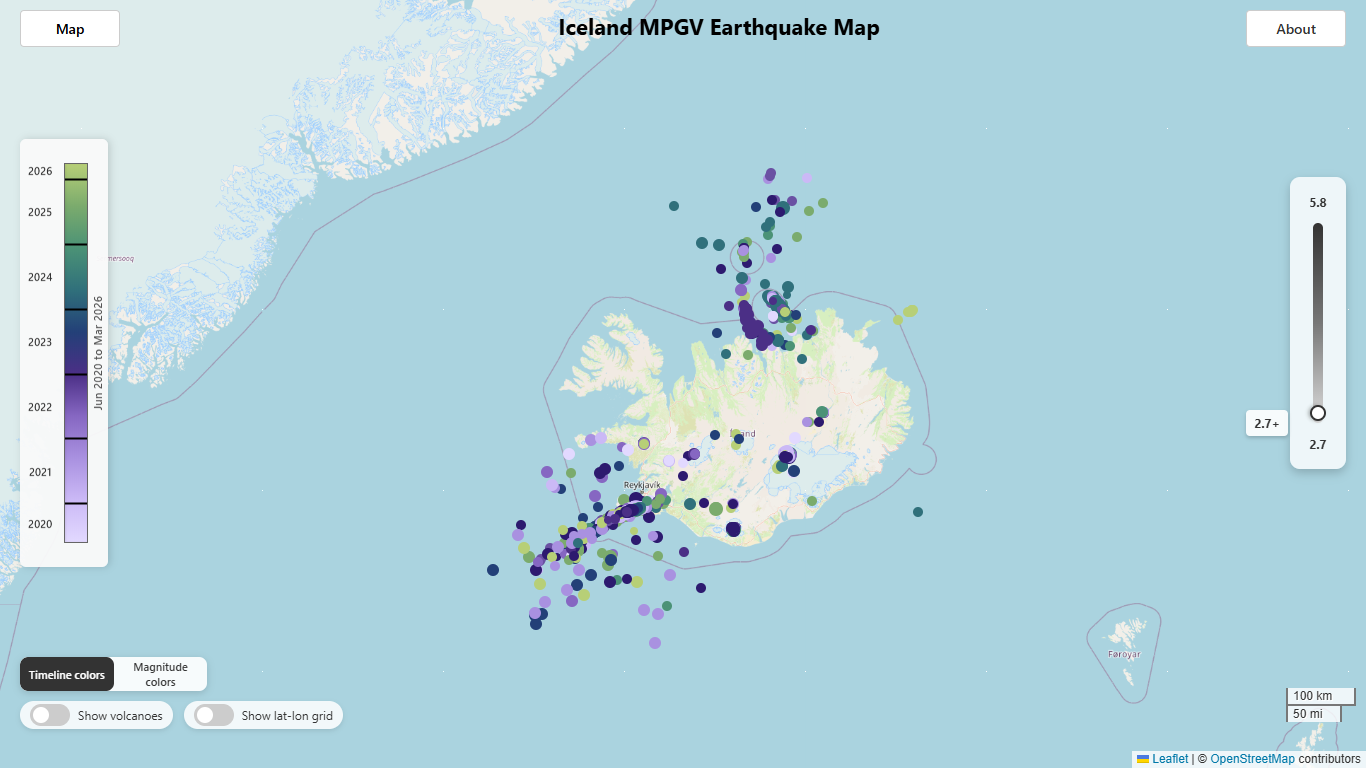
\includegraphics[width=\linewidth]{Screenshots/Webapp_front.png}
\caption{Main frontend interface of MPGV Monitor showing the interactive Leaflet map view, temporal filtering controls, magnitude scale, and optional overlays.}
\end{figure}


\subsection{Frontend Codebase Structure}
\label{subsec:frontend_structure}

The frontend is organized into a small number of entry files and a set of UI components. The following files form the structural backbone:

\begin{itemize}
    \item \texttt{main.jsx}: application entry point that mounts React into the HTML root.
    \item \texttt{App.jsx}: top-level coordinator responsible for global state and orchestration.
    \item \texttt{api.js}: a dedicated communication layer used to fetch data from backend endpoints.
    \item \texttt{App.css} and \texttt{index.css}: global styling and baseline layout behavior.
\end{itemize}

The \texttt{components/} directory contains focused UI modules that map directly to visible interface controls and overlays:

\texttt{MapComponent.jsx} (map rendering and marker management), 
\texttt{MapTypeSelector.jsx} (basemap selection), 
\texttt{TimeWindowSlider.jsx} (temporal filtering),
\texttt{MagnitudeScale.jsx} (magnitude threshold and legend),
\texttt{VolcanoMarker.jsx} (volcano overlay rendering)
and \texttt{About.jsx} (modal information panel).

This decomposition ensures each component has a clear responsibility, while \texttt{App.jsx} remains the single point where global state is stored and propagated.


\subsection{Leaflet Integration and Tile Layer Architecture}
\label{subsec:frontend_leaflet}

The spatial rendering layer uses Leaflet~1.9, an open-source JavaScript mapping library, integrated into React through the \texttt{react-leaflet}~4.2 bindings. This replaces the Google Maps JavaScript API that was used in a previous version of the frontend. Leaflet was chosen because it is open-source, requires no API key, has a large plugin ecosystem, and handles custom overlays and canvas-based rendering well.

Unlike Google Maps, which requires a paid API key and imposes usage-based billing, Leaflet operates with freely available tile services. No credentials, environment variables, or cloud-based key management are required. This eliminates the \texttt{.env} file dependency that was present in the Google Maps version and simplifies deployment across development and production environments.

The \texttt{TileLayerManager} subcomponent within \texttt{MapComponent.jsx} selects the appropriate tile source based on the active map mode:

\begin{table}[H]
\centering
\begin{tabular}{l l l}
\hline
\textbf{Map Mode} & \textbf{Tile Provider} & \textbf{Cost} \\
\hline
Roadmap   & OpenStreetMap             & Free (open data) \\
Satellite & Esri World Imagery        & Free tier \\
Dark Mode & CartoDB Dark Matter       & Free tier \\
Heatmap   & CartoDB Dark Matter (no labels) + label pane & Free tier \\
\hline
\end{tabular}
\caption{Tile providers used for each basemap mode in the Leaflet-based frontend.}
\label{tab:tile-providers}
\end{table}

\vspace{0.7cm}

\begin{figure}[H]

\centering    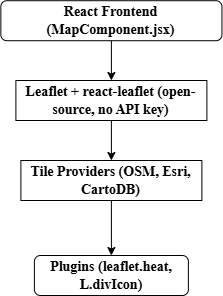
\includegraphics[width=0.4\textwidth, height=8cm]{Screenshots/Frontend integration.png}
\caption{Frontend integration with the Leaflet mapping library, illustrating the open-source tile provider architecture that replaces the previous Google Maps API dependency.}
\end{figure}

Tile layer performance is optimized through several Leaflet-specific configuration options: \texttt{updateWhenZooming=false} prevents tile reloading during zoom animations, \texttt{keepBuffer=4} pre-loads surrounding tiles to reduce blank areas during panning, and \texttt{detectRetina=false} avoids doubled tile requests on high-DPI displays. The map is configured with \texttt{preferCanvas=true}, which routes marker rendering through the HTML5 Canvas API rather than SVG, providing 3--5$\times$ faster redraws when displaying thousands of earthquake markers.

\subsection{Backend Connection}
\label{subsec:frontend_api_layer}

A central design decision in MPGV Monitor is that the frontend does not communicate with the database directly. Instead, the backend exposes curated data through a stable set of HTTP endpoints (e.g., \texttt{/earthquakes}, \texttt{/volcanoes}, and ShakeMap-related routes). The frontend uses a single communication module, \texttt{api.js}, as the exclusive gateway to these endpoints.

Centralising all HTTP calls in one file means that if the backend URL changes or error handling needs updating, only \texttt{api.js} is touched. Components call \texttt{fetchEarthquakeData()} or \texttt{fetchVolcanoData()} without knowing or caring about URL paths or response formats.

\paragraph{Example (minimal API abstraction).}
A representative pattern used in \texttt{api.js} is:

\begin{verbatim}
export async function fetchEarthquakeData() {
  const response = await axios.get(`${API_URL}/earthquakes`);
  return response.data;
}
\end{verbatim}

In practice, similar functions exist for volcano metadata and optional ShakeMap resources. The key point is architectural: UI components call stable functions such as \texttt{fetchEarthquakes()} rather than repeating request logic throughout the codebase.

\vspace{0.7cm}

\begin{figure}[H]

\centering    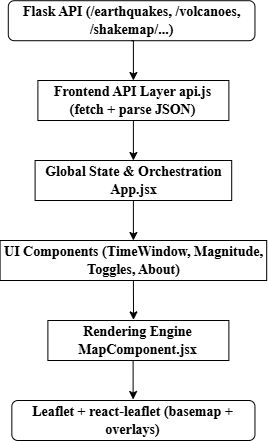
\includegraphics[width=0.4\textwidth, height=10cm]{Screenshots/Frontend data flow.png}
\caption{Frontend data flow from backend API endpoints through \texttt{api.js} into global state management in \texttt{App.jsx}, and onward to UI controls and Leaflet-based map rendering.}
\end{figure}

\subsection{Top-Level Orchestration}
\label{subsec:frontend_app}

The \texttt{App.jsx} component is the coordinator of the frontend. It is responsible for:

(1) loading datasets using \texttt{api.js}; 
(2) storing global UI state (filters, toggles, selected event, color mode); 
and (3) distributing state and callbacks to child components.

This design follows a state-lifting approach: shared state lives at the highest common ancestor so that changes in one control (e.g., the magnitude slider) can consistently update other parts of the interface (e.g., the map markers and the event inspection panel).

At runtime, \texttt{App.jsx} performs an initial data fetch when the application loads. Earthquakes are requested from the backend and stored as an in-memory dataset used for map rendering. Volcano metadata is fetched similarly (if enabled in the UI flow). Because the backend performs reconciliation and produces a unified catalogue, the frontend can treat the dataset as authoritative and focus on interactive operations (filtering and encoding) without additional validation steps.

The orchestration role of \texttt{App.jsx} is also visible through callbacks: when the user adjusts the time window or magnitude threshold, the corresponding component reports changes upward through a function prop. \texttt{App.jsx} updates state, and React’s reactivity triggers downstream updates.

\subsection{Map Rendering and Marker Lifecycle}
\label{subsec:frontend_mapcomponent}

The map rendering logic is implemented in the \texttt{MapComponent.jsx} module (approximately 650 lines), which acts as the spatial rendering engine of the frontend. It is responsible for constructing the Leaflet map instance and managing the lifecycle of all map overlays. Unlike static map outputs, this component must support dynamic re-rendering of markers when filters, color mode, or overlays change.

\paragraph{Map initialization.}
Upon mounting, \texttt{MapComponent.jsx} initializes a Leaflet map via the \texttt{react-leaflet} \texttt{<MapContainer>} component. The initial configuration sets a default center at approximately $64.96^{\circ}$\,N, $-19.02^{\circ}$\,W with zoom level~6, appropriate for a full-Iceland view. The map is configured with \texttt{preferCanvas=true} for canvas-accelerated rendering, \texttt{zoomSnap=0.5} and \texttt{zoomDelta=0.5} for half-step zoom increments, and \texttt{minZoom=5.5} to prevent users from zooming out beyond Iceland's context. A \texttt{MapReadyHandler} subcomponent calls \texttt{map.invalidateSize()} after 150\,ms to ensure correct sizing after CSS layout completion.

\paragraph{Marker creation and updates.}
Earthquake markers are rendered as square-shaped SVG symbols using Leaflet's \texttt{L.divIcon} API. Each marker's icon is an inline SVG element whose size and color are computed from magnitude and the active color mode. Marker pixel sizes follow a sublinear growth function:

\[
\text{px} = \text{round}\!\left(8 + \left(\frac{M_w - 2.7}{M_{w,\max} - 2.7}\right)^{0.7} \times 6\right)
\]

yielding sizes from 8\,px (smallest events) to 14\,px (largest). The exponent of 0.7 ensures that small-magnitude events cluster tightly while large events receive proportionally more visual weight.

All earthquake markers are managed through a single \texttt{L.layerGroup}, enabling $O(1)$ show/hide operations for the entire layer. This is a significant performance improvement over the Google Maps version, which required iterating through individual markers. Marker objects are stored in a \texttt{Map<quakeKey, \{marker, quake, index\}>} structure, and when the selected earthquake changes, only the two affected markers (previous and new selection) are updated rather than the entire collection.

\paragraph{Color encoding.}
Two color modes are supported:

\begin{itemize}
    \item \textbf{Timeline mode:} markers are colored by month using a 12-stop twilight palette ranging from light purple (January) through dark indigo (summer) to green (December). The color is determined by \texttt{date.getUTCMonth()}.
    \item \textbf{Magnitude mode:} markers are colored using a 5-stop viridis-like palette from yellow ($M_{w,\min}$) through green and teal to deep purple ($M_{w,\max}$), interpolated linearly based on the normalized magnitude.
\end{itemize}

\paragraph{Event selection and the information panel.}
Clicking a marker triggers a selection action. The selected marker receives a white stroke and a 4\,px size boost to distinguish it visually. An information panel appears showing magnitude, depth, event time, latitude, longitude, and, if a validated ShakeMap association exists, a button linking to the EPOS ShakeMap product. The ShakeMap lookup is performed asynchronously via \texttt{fetchShakeMapValidated()}.

The information panel is intentionally ephemeral. It closes automatically after 15 seconds and also closes immediately if the user changes time or magnitude filters or clicks the map background. This behavior prevents the UI from displaying details that no longer correspond to the currently visible filtered dataset.

\paragraph{Heatmap visualization.}
The heatmap mode, introduced in the Leaflet version, uses the \texttt{leaflet.heat} plugin to render a density-based heat overlay. Each earthquake contributes a point with a base weight of 1.0, boosted to 1.15 for events with $M_w \geq 4.0$ and 1.3 for $M_w \geq 5.0$. The heatmap radius is zoom-responsive (15--58\,px) and uses a custom gradient transitioning through dark blue, teal, amber, and red. The heatmap layer rebuilds only on data changes or zoom events; panning is free, maintaining approximately 60\,FPS.

\begin{figure}[H]
\centering
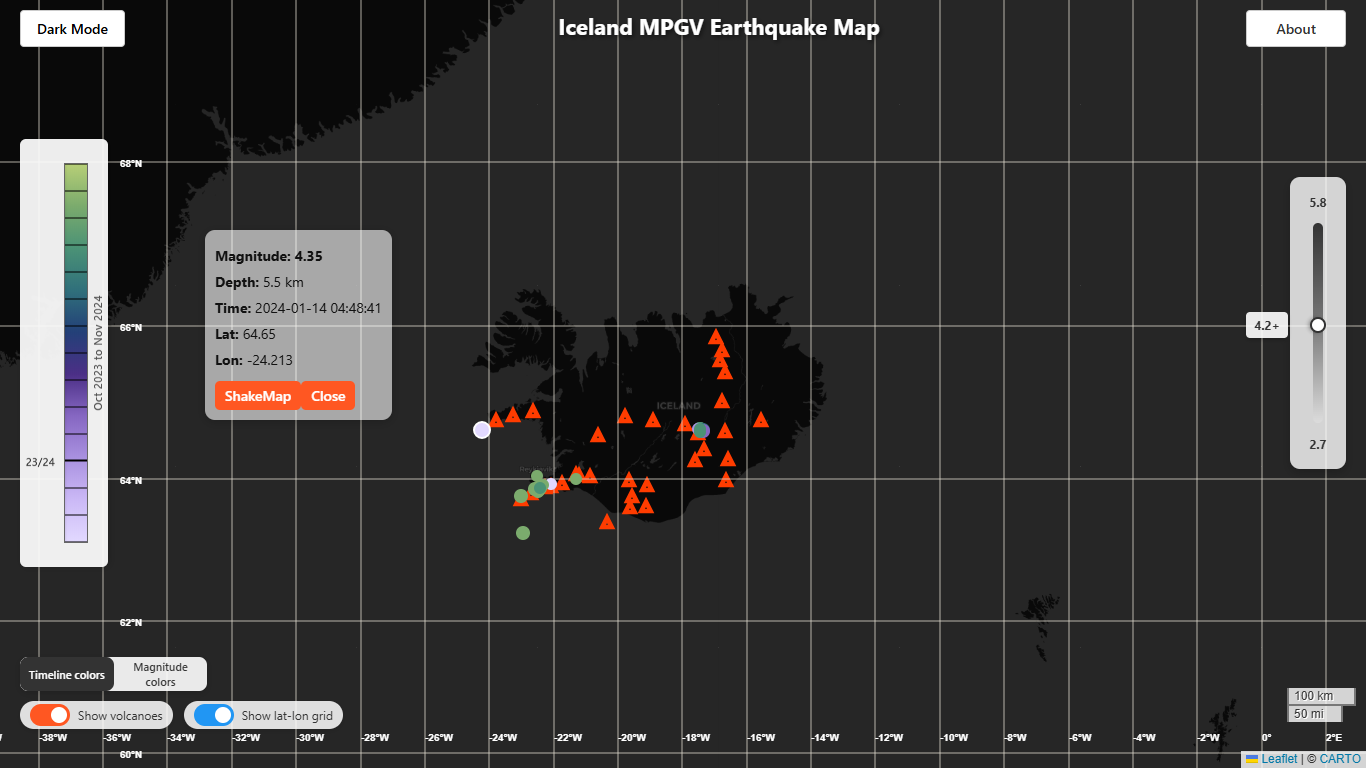
\includegraphics[width=\linewidth]{Screenshots/info_window.png}
\caption{Event inspection panel displayed after marker selection, showing magnitude, time, depth, coordinates, and optional ShakeMap linkage. Volcano markers and the latitude/longitude grid overlay are also visible.}
\end{figure}


\subsection{Basemap Selection}
\label{subsec:frontend_maptypeselector}

The basemap selector provides four modes: standard roadmap (OpenStreetMap), satellite imagery (Esri World Imagery), a dark theme (CartoDB Dark Matter), and a density-based heatmap (CartoDB Dark Matter with a label overlay pane). This represents an expansion from the three modes available in the previous Google Maps version, with the heatmap being a new addition enabled by the Leaflet plugin ecosystem.

From an architectural standpoint, this component does not manage map state directly. Instead, it emits the selected map mode to \texttt{App.jsx}, which updates the global state. \texttt{MapComponent.jsx} then applies the correct tile layer configuration through the \texttt{TileLayerManager} subcomponent.

Keeping the selector ignorant of tile URLs and map state avoids tight coupling and makes the component easy to test in isolation: it only has to emit a string, and \texttt{MapComponent.jsx} handles the rest.

\subsection{Temporal Filtering}
\label{subsec:frontend_timewindow}

The TimeWindow slider supports exploration across multiple temporal resolutions. At a high level, the slider enables the user to restrict the visible earthquake catalogue to a selected interval. What distinguishes this control from a basic date picker is its multi-scale behavior: the slider presents coarse year-level ranges when zoomed out, and transitions into month-level and day-level resolution as the user zooms in.

The idea is that a seismologist browsing five years of data and a civil-protection officer zooming into yesterday's swarm need different temporal granularity, and the slider should handle both without a mode switch. Internally, the component reports the selected interval to \texttt{App.jsx} through a callback, and the filtered interval is applied when deriving the marker set shown on the map.

The temporal slider also interacts with color encoding. When timeline-color mode is enabled, marker colors reflect temporal progression across the active dataset (e.g., older to newer). When magnitude-color mode is enabled, the time slider remains functional as a filter but is visually muted to indicate that it is not the active encoding dimension.

\subsection{Magnitude Thresholding}
\label{subsec:frontend_magnitude}

The MagnitudeScale component provides a vertical threshold slider that ranges from the system’s minimum magnitude (filtered at ingestion to $Mw \geq 2.7$) to the maximum magnitude observed in the current dataset. The selected threshold defines which events remain visible. This filter is critical for exploring swarms: users can suppress smaller events to highlight only stronger earthquakes.

In magnitude-color mode, the component also acts as a legend. Marker colors correspond to magnitude intensity, enabling quick interpretation of spatial distributions of event strength. In timeline-color mode, the magnitude scale remains active as a filter but is visually muted, reinforcing the separation between \emph{filtering} and \emph{encoding mode}.

\paragraph{Example (mode-dependent color selection).}
A short illustrative snippet is sufficient:

\begin{verbatim}
const color = (mode === "magnitude")
  ? magnitudeColor(event.mw)
  : timelineColor(event.time);
\end{verbatim}

The thesis emphasis is the interaction logic: a single dataset supports multiple analytical encodings through a mode switch rather than duplicating rendering pipelines.

\subsection{Volcano Overlay}
\label{subsec:frontend_volcano}

The volcano overlay is a supplementary spatial layer that can be toggled on and off. When enabled, volcano markers are rendered as distinct orange/red triangle symbols (20$\times$20\,px SVG icons), visually separated from the square earthquake markers. This layer supports contextual interpretation: clusters of seismicity can be compared against known volcanic systems.

From an architectural perspective, \texttt{VolcanoMarker.jsx} uses Leaflet's imperative API via the \texttt{useMap()} hook from \texttt{react-leaflet}, creating \texttt{L.marker} instances with custom \texttt{L.divIcon} SVG icons directly on the map. This imperative approach was chosen because it provides finer control over marker lifecycle than the declarative \texttt{react-leaflet} \texttt{<Marker>} component. Each volcano marker is manually cleaned up on unmount via \texttt{map.removeLayer(marker)}. The component renders no JSX and returns \texttt{null}.

\subsection{Latitude/Longitude Grid Overlay}
\label{subsec:frontend_grid}

The latitude/longitude grid overlay is an optional aid for spatial orientation. When enabled, the map displays a grid of reference lines across the full view, implemented using \texttt{L.polyline} for grid lines and \texttt{L.marker} with \texttt{L.divIcon} for coordinate labels. This control is particularly useful when users want approximate spatial comparisons without continuously referencing the coordinates in the inspection panel.

The grid is \textbf{zoom-responsive}: the spacing and label precision adapt automatically as the user zooms in or out. At low zoom levels ($z < 5$), grid lines are spaced at $5^{\circ}$ intervals with zero decimal places; at high zoom levels ($z \geq 15$), the spacing narrows to $0.01^{\circ}$ with four decimal places. Intermediate levels introduce both major and minor (sub-)grid lines for improved readability. The grid rebuilds on \texttt{zoomend} and \texttt{moveend} events.

A \textbf{safe-zone calculation} ensures that latitude labels never overlap the TimeWindow slider panel on the left side of the interface: labels positioned less than 120\,px from the left edge of the viewport are suppressed. Grid line and label colors adapt automatically to the active basemap (light or dark theme).

As with the volcano overlay, the grid is controlled via a toggle in the interface. The overlay is treated as auxiliary and does not change earthquake filtering or encoding.

\subsection{About Modal}
\label{subsec:frontend_about}

The About panel is a modal overlay that explains the system and its data sources. Opening it does not touch the map state, filters, selected markers, and overlays remain exactly as they were, so users can check what the tool does without accidentally resetting their analysis.

\subsection{State Interaction Model and Cross-Component Consistency}
\label{subsec:frontend_state_model}

With several controls all affecting the same map, the main risk is inconsistency: a user changes the time window, but the info panel still shows a marker that no longer passes the filter. All shared state lives in \texttt{App.jsx}, and a few explicit rules keep things coherent:

\begin{itemize}
    \item \textbf{Filter changes invalidate inspection context:} changing the time window or magnitude threshold clears the selected event and closes the information panel.
    \item \textbf{Encoding mode is explicit:} a single toggle determines whether color encodes time or magnitude. The inactive legend/scale is visually muted to reduce ambiguity.
    \item \textbf{Overlay toggles are independent:} volcano markers and the grid can be enabled without affecting filtering.
    \item \textbf{Basemap changes preserve analytical state:} switching Map/Satellite/Dark changes cartographic context but does not reset filters or marker selection.
\end{itemize}

The net effect is that the map never lies: what the user sees always matches the active filter and encoding settings.

\subsection{Rendering Pipeline and Performance Considerations}
\label{subsec:frontend_performance}

Rendering several thousand markers in a browser without visible lag requires some care. The approach used here is a straightforward pipeline: fetch data once, derive a filtered subset, compute colour and size for each surviving event, and update only the affected overlays.

The migration from Google Maps to Leaflet introduced several performance optimizations that were not available in the previous version:

\begin{table}[H]
\centering
\begin{tabular}{l l l}
\hline
\textbf{Component} & \textbf{Technique} & \textbf{Benefit} \\
\hline
EarthquakeMarkers & Single \texttt{L.layerGroup} & $O(1)$ show/hide \\
Selection change  & Update only 2 markers & $O(1)$ vs $O(n)$ \\
Marker icons      & \texttt{useMemo} on deps & Avoid per-render recalculation \\
Tile loading      & \texttt{updateWhenZooming=false} & Smooth zoom, fewer blanks \\
Tile buffering    & \texttt{keepBuffer=4} & Pre-loaded surrounding tiles \\
Heatmap           & Rebuild on data/zoom only & Panning is free ($\sim$60\,FPS) \\
Canvas rendering  & \texttt{preferCanvas=true} & 3--5$\times$ faster redraws \\
Zoom animation    & \texttt{zoomSnap=0.5} & Half-step snapping, smoother UX \\
TimeWindow slider & Stable wheel handler via \texttt{useRef} & No listener re-registration \\
\hline
\end{tabular}
\caption{Frontend performance optimizations in the Leaflet-based architecture.}
\label{tab:frontend-perf}
\end{table}

A practical performance consideration is avoiding expensive full reinitialization of the map. The Leaflet map instance is created once, and subsequent interactions update only the affected overlays. Data filtering occurs before rendering marker objects, which limits the number of overlays created when the user narrows time windows or raises the magnitude threshold.

\subsection{Comparison with Existing Seismic Web Applications}
\label{subsec:frontend_comparison}

MPGV Monitor is not trying to replace global catalogues or real-time alert services. Its niche is Iceland-specific analytical exploration backed by a reconciled, multi-source catalogue. To make that positioning concrete, it helps to compare against what already exists.

\paragraph{Iceland-focused platforms.}
The IMO earthquake page shows epicentres from roughly the last 48~hours alongside a table and supporting plots \cite{imo_quakes_48h}. It is authoritative and immediately readable, but a researcher who wants to study how the Reykjanes swarm evolved over 2021--2024 has no temporal slider to work with. earthquakes.is \cite{earthquakes_is} fills a similar real-time niche with a simpler interface geared toward public monitoring. Neither service reconciles multiple catalogues or links events to ShakeMap products. MPGV Monitor keeps the map-first immediacy of these tools but adds multi-year temporal navigation, magnitude thresholding, dual colour encodings, and a backend that algorithmically matches MPGV and Skjálftalísa records before anything reaches the screen.

\paragraph{Global platforms.}
The USGS Latest Earthquakes application \cite{usgs_latest_map} covers the entire planet with standardized reporting and event-detail pages, an interface that has to work for Tokyo and Reykjavik alike. EMSC \cite{emsc_home,emsc_map} adds a ``citizen seismology’’ layer, incorporating crowdsourced felt-reports alongside institutional data. The IRIS Interactive Earthquake Browser \cite{iris_ieb_app,iris_ieb_help} targets researchers and educators, offering large-scale querying and CSV export over a Google Maps base. All three are valuable, but none is specialized for Iceland’s data landscape. MPGV Monitor trades global breadth for domain depth: because the backend already knows about MPGV page layouts, Skjálftalísa JSON schemas, and EPOS ShakeMap endpoints, the frontend can offer interactions, volcano overlays, ShakeMap drill-down, heatmap mode, that a general-purpose viewer cannot justify building.

\paragraph{Where MPGV Monitor sits.}
Table~\ref{tab:seismic_comparison} summarizes the comparison. The common thread across existing platforms is that they are optimized either for rapid public awareness (IMO, earthquakes.is, EMSC) or for broad research querying (USGS, IRIS). MPGV Monitor occupies a middle ground: analytical depth within a specific geographic and institutional context, with a data pipeline that reconciles sources and links events to downstream intensity products before anything is rendered. The Leaflet migration reinforced this position by removing the API-key cost of Google Maps and enabling features, canvas-accelerated rendering, density heatmaps, a zoom-responsive grid, that were not feasible under the previous stack.

\begin{table}[h]
\centering
\small
\begin{tabular}{p{3cm} p{2.5cm} p{2.5cm} p{3cm} p{3cm}}
\hline
\textbf{Platform} & \textbf{Scope} & \textbf{Purpose} & \textbf{Strengths} & \textbf{Limitations} \\
\hline

IMO & Iceland (48h focus) & Public reporting & Official authoritative data; rapid overview & Limited long-term analytical tools \\

earthquakes.is & Iceland & Live monitoring & Real-time tracking; simple interface & No explicit multi-source reconciliation \\

USGS & Global & Global reporting & Global coverage; standardized products & Not region-specialized for Iceland \\

EMSC & Global & Rapid dissemination & Citizen seismology integration & Public-response oriented \\

IRIS IEB & Global & Research/education & Large-scale querying; export tools & Not product-linked to Icelandic ShakeMaps \\

\textbf{MPGV Monitor} & Iceland (multi-year) & Analytical exploration & Reconciled catalogue; ShakeMap linkage; dual encoding; temporal zoom; heatmap; no API key & Region-specific scope \\

\hline
\end{tabular}
\caption{Comparison of MPGV Monitor with Selected Seismic Web Applications}
\label{tab:seismic_comparison}
\end{table}

Table~\ref{tab:seismic_comparison} summarizes the positioning of MPGV Monitor relative to established earthquake web platforms. While global systems prioritize breadth of coverage and public dissemination, MPGV Monitor emphasizes depth within a specific geographic domain through multi-source reconciliation and analytical interaction design.


\subsection{Summary}
\label{subsec:frontend_summary}

Taken together, the frontend replaces the earlier Google Maps dependency with a Leaflet-based map that pulls its tiles from three free providers (OpenStreetMap, Esri World Imagery, CartoDB Dark Matter) and talks to the backend exclusively through \texttt{api.js}. Users can filter by time at multiple resolutions, set a magnitude threshold, switch marker colour between timeline and magnitude encoding, toggle a density heatmap, and overlay volcano markers or a lat/lon grid, all without the backend needing to know which view is active. Canvas rendering, layer-group visibility toggling, and memoised icon computation keep the interface responsive even when several thousand markers are on screen. The practical upshot is an analytical map that costs nothing to serve, stays snappy under load, and leaves every data decision to the backend.


% ============================ CHAPTER 7 ============================
\section{Final Features}
\subsection{Final Feature Polishing}
Once the core Leaflet migration was functionally complete, a separate polishing phase addressed the rough edges that only become visible through sustained daily use and informal user testing. This section documents the main refinements, the reasoning behind them, and the trade-offs involved.

\subsubsection{Heatmap Gradient and Radius Tuning}

The initial heatmap implementation used a single fixed radius, which looked acceptable at the default zoom level but produced either a featureless blur (zoomed out) or isolated blobs (zoomed in). After experimenting with several radius--zoom mappings, a lookup table was adopted that scales the point radius with the zoom level:

\begin{table}[H]
\centering
\small
\begin{tabular}{l c c c c c c}
\hline
\textbf{Zoom} & 5 & 6 & 7 & 8 & 9 & 10+ \\
\textbf{Radius (px)} & 15 & 22 & 30 & 38 & 48 & 58 \\
\hline
\end{tabular}
\caption{Heatmap radius values at representative zoom levels.}
\label{tab:heatmap-radii}
\end{table}

The gradient was also redesigned from a generic red--yellow ramp to a four-stop scale (transparent $\rightarrow$ blue $\rightarrow$ yellow $\rightarrow$ red) that gives a clearer visual separation between low-density background and high-density clusters such as the Reykjanes swarms.

\subsubsection{Latitude/Longitude Grid Overlay}

The grid overlay draws degree lines across the visible map extent and labels them along the edges. Two problems surfaced during testing. First, at certain zoom levels the labels overlapped with the TimeWindow slider on the left side of the screen. This was solved by defining a ``safe zone'' in pixel coordinates: labels whose screen position falls inside the slider's bounding box are simply not drawn. Second, the label text was hard to read against both light and dark tile layers. Adding a thin white halo (CSS \texttt{text-shadow}) around each label made them legible on all four basemaps without requiring per-layer colour logic.

\subsubsection{Marker Rendering Performance}

With the full dataset loaded (1\,781 merged events), the original SVG-based markers caused noticeable lag during panning and zooming on mid-range hardware. Three changes brought the frame rate back to acceptable levels:

\begin{enumerate}
    \item \textbf{Canvas acceleration.} Setting \texttt{preferCanvas: true} on the Leaflet map instance routes all vector rendering through a single \texttt{<canvas>} element rather than creating individual DOM nodes per marker.
    \item \textbf{Layer-group visibility.} Instead of adding and removing markers from the map on every filter change, all markers are placed in a \texttt{L.layerGroup} at load time. Filtering then toggles the group's visibility, an O(1) operation, rather than iterating through thousands of individual layers.
    \item \textbf{Memoised icon computation.} Each earthquake marker's \texttt{L.divIcon} is generated by a function that caches its output based on magnitude band and colour mode. This avoids regenerating identical SVG strings on every render cycle.
\end{enumerate}

\subsubsection{Z-Index Alignment}

Leaflet's internal pane system assigns z-index values in the 400--700 range by default, which is significantly higher than Google Maps' defaults. After the migration, several UI controls (the About button, the map-type selector, the magnitude scale) rendered \emph{behind} the tile pane. Fixing this required raising the z-index of \texttt{.controls} and \texttt{.about-button-container} to 1001 and the magnitude scale to 1000, values that sit safely above Leaflet's highest default pane (overlay pane at 400) while still leaving room for pop-ups and tooltips.

\subsubsection{CSV Export}

A recurring request during informal testing was the ability to download the displayed earthquake data for use in external tools (Excel, MATLAB, R). A new backend endpoint, \texttt{/earthquakes\_csv}, serialises the merged catalogue as a comma-separated file with headers matching the JSON field names. The About modal in the frontend provides a download link that hits this endpoint, so users can export whatever subset the current time and magnitude filters define.

\subsubsection{User Feedback and Interface Adjustments}

Several smaller changes came directly from watching users interact with the application during informal testing sessions:

\begin{itemize}
    \item The TimeWindow slider was moved slightly inward from the left edge after users on smaller screens reported that it overlapped the zoom controls.
    \item The default colour palette for timeline-based marker colouring was adjusted after feedback that the original green-to-red ramp was hard to distinguish for users with red--green colour deficiency.
    \item The overall interface layout was tightened so that the map occupies the maximum possible screen area, with controls kept compact and positioned along the edges rather than floating over the map centre.
\end{itemize}

These adjustments were minor individually, but collectively they made the difference between a prototype that worked and an interface that felt ready to show to external stakeholders.

\newpage

% ============================ CHAPTER 8 ============================
\section{Deployment, Testing \& Debugging}
\subsection{Backend \& Frontend Testing}
Extensive testing was carried out on both the backend and frontend. The backend test suite, executed via \texttt{python -m pytest tests/ -v}, includes 40 passing tests across five test files:

\begin{itemize}
    \item \texttt{test\_haversine.py}: 10 tests for the \texttt{haversine\_km()} pure function, covering identical points, threshold boundary behaviour, and real Iceland locations.
    \item \texttt{test\_scrape\_parse.py}: 14 tests for MPGV HTML table parsing with mocked HTTP responses, verifying magnitude filtering and timestamp normalization.
    \item \texttt{test\_reconcile.py}: 13 integration tests for the \texttt{match\_and\_merge()} reconciliation algorithm, covering unique matches, ambiguous multi-candidate scenarios, unmatched events, and depth policy enforcement.
    \item \texttt{test\_volcano\_scraper.py}: 3 tests for the EPOS volcano metadata ingestion module, covering the primary API endpoint, the v1 fallback path, and the empty-response case.
    \item \texttt{test\_volcano\_scraper\_live.py}: 1 live integration test that queries the real EPOS volcano API, skipped by default to avoid depending on external service availability.
\end{itemize}

Test isolation is achieved through a \texttt{conftest.py} fixture that sets \texttt{DISABLE\_SCHEDULER}, redirects the database to a temporary file, and rebuilds the SQLAlchemy engine for each test session.

The frontend test suite uses Vitest with \texttt{@testing-library/react} and a jsdom environment. It contains 12 tests for the \texttt{TimeWindowSlider} component, covering basic rendering, year-mode label positioning, callback behaviour, and month-mode label formatting. The frontend tests are executed via \texttt{npm test} from the \texttt{frontend/} directory.

In addition to automated tests, manual user testing was conducted with sample users to evaluate UI responsiveness, data accuracy, and the usability of the Leaflet-based map interface following the migration from Google Maps.


\subsection{Early Deployment Testing (Historical)}

During an earlier phase of development, a preliminary deployment was carried out on the university's Pluto server to validate that the application could run in a networked environment. This deployment used the previous Google Maps--based version of the frontend and served primarily as a proof-of-concept exercise. It is no longer active and does not reflect the current Leaflet-based architecture; however, the experience informed several deployment decisions documented below.

\subsubsection{Setup and Challenges}
The application was hosted using \texttt{gunicorn}, a production-ready WSGI server, behind the server's public IP address on port~7000. Initial attempts encountered issues with Python path resolution (\texttt{ModuleNotFoundError}) and port conflicts when \texttt{gunicorn} was invoked without the correct working directory. These were resolved by explicitly setting the \texttt{--chdir} flag and activating the virtual environment before launching the server.

The final working command ran \texttt{gunicorn} in the background using \texttt{nohup}:

\begin{verbatim}
nohup gunicorn -b 0.0.0.0:7000 backend.app:app \
  --chdir ~/QuakeMap > gunicorn.log 2>&1 &
\end{verbatim}

The application was then accessible at \texttt{http://130.208.113.169:7000/} and responded correctly to HTTP requests.

\begin{figure}[H]
    \centering
    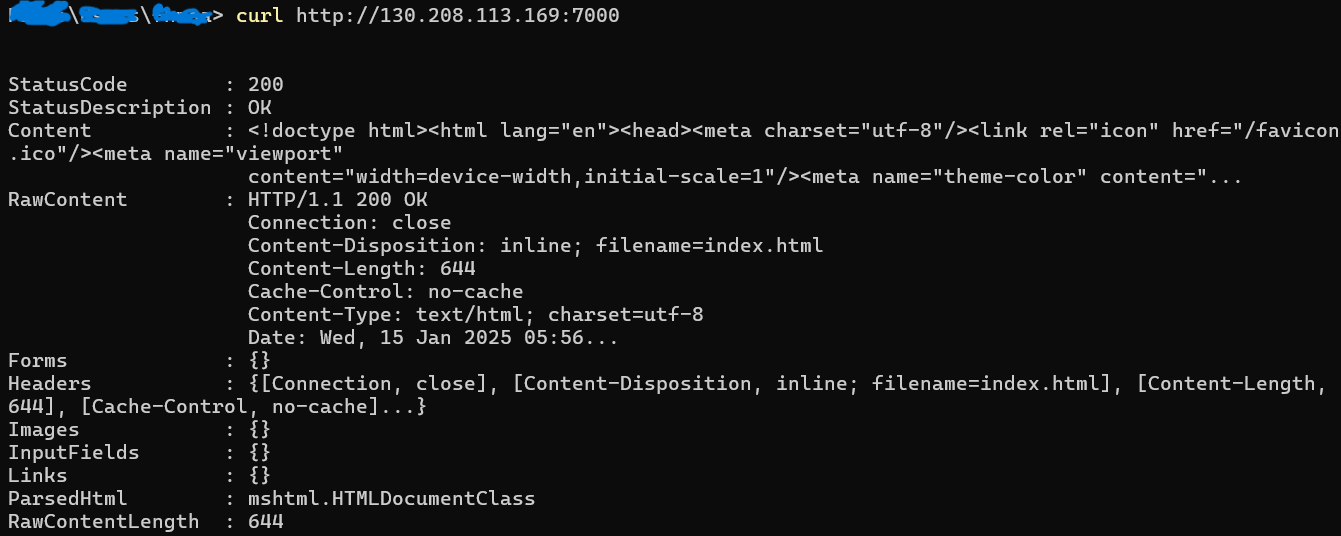
\includegraphics[width=\linewidth]{Screenshots/Deployment_Testing.png}
    \caption{Confirmation of the early Pluto server deployment responding to HTTP requests (historical; this deployment is no longer active).}
\end{figure}

\subsubsection{Lessons Learned}
This early deployment highlighted several practical considerations:

\begin{itemize}
    \item Proper configuration of the working directory and Python path is critical for \texttt{gunicorn}.
    \item Background execution via \texttt{nohup} is a pragmatic solution in environments with limited permissions, but lacks automatic restart and robust logging compared to process managers such as \texttt{systemd}.
    \item The absence of load balancing and crash recovery mechanisms made the setup unsuitable for sustained public-facing use.
\end{itemize}

These lessons directly inform the planned production deployment strategy described below.

\subsection{Planned Production Deployment}

The current Leaflet-based version of MPGV Monitor is under active development and has not yet been deployed to a production server. The planned deployment will proceed in two stages:

\begin{enumerate}
    \item \textbf{Internal testing deployment:} The application will first be deployed to a local university or institutional server for internal review, performance validation, and user acceptance testing. This stage will use a production-grade WSGI server (such as \texttt{gunicorn} behind a reverse proxy like \texttt{nginx}) together with a process manager (\texttt{systemd}) for automatic restart and log management.
    \item \textbf{Public production deployment:} Following successful internal testing, the application is intended to be deployed for public access through the Icelandic Meteorological Office (IMO). This deployment will require addressing tile provider licensing (see Section~\ref{subsec:tile_licensing}), configuring HTTPS, and ensuring the system meets the operational requirements for a publicly accessible monitoring tool.
\end{enumerate}

The modular architecture of MPGV Monitor, with a stateless Flask API backend and a static-asset React frontend, is well suited to standard deployment patterns. The frontend can be served as a pre-built static bundle via \texttt{nginx} or a CDN, while the backend can run as a persistent \texttt{gunicorn} process with the SQLite database on local storage.

\subsection{Model Deployment}
Once a predictive model is developed (see Section~\ref{subsec:prediction_model}), it will be integrated into the backend and exposed through a dedicated API endpoint, enabling users to query predicted seismic activity in real time through the frontend interface.

% ============================ CHAPTER 9 ============================
\section{Future Development}

MPGV Monitor now handles the core loop, pulling data in, reconciling it, and letting users explore the result on a map, but a number of directions remain open. Some of these came up during user testing, others emerged from conversations with staff at the Icelandic Meteorological Office, and a few reflect longer-term research goals that go beyond what a single thesis can cover. The subsections below describe the ones I consider most promising.

\subsection{Accessibility and Inclusive Design}

The current interface assumes mouse-driven interaction and does not yet meet formal accessibility standards. WCAG~2.1 \cite{WCAG21} organises its guidance around four principles, perceivable, operable, understandable, and robust, each of which points to concrete gaps in the existing frontend.

Planned accessibility enhancements include:

\begin{itemize}
    \item \textbf{Keyboard navigation:} Ensuring that all interactive controls, including the TimeWindow slider, magnitude scale, map type selector, and overlay toggles, are fully operable via keyboard input, without requiring a mouse or touch interaction. This is particularly important for users with motor impairments who rely on keyboard-only navigation or assistive switch devices.
    \item \textbf{Screen reader compatibility:} Adding ARIA (Accessible Rich Internet Applications) labels and roles to map markers, information panels, and interactive controls so that screen reader software can convey the interface structure and earthquake data to visually impaired users \cite{WAI_ARIA}. This includes providing text alternatives for the SVG-based earthquake and volcano marker icons.
    \item \textbf{High-contrast and colorblind-safe modes:} Introducing alternative color palettes designed to remain distinguishable for users with color vision deficiencies (such as deuteranopia and protanopia). Research on colorblind-safe visualization palettes, such as the work by Brewer \cite{Brewer2003ColorBrewer}, provides established guidance for selecting color schemes that maintain perceptual distinctness across common forms of color blindness.
    \item \textbf{Text scaling and readability:} Ensuring that all text elements (labels, legends, information panels) respect browser-level font size preferences and remain readable when scaled up to 200\%, in accordance with WCAG Success Criterion~1.4.4.
    \item \textbf{Focus management:} Implementing visible focus indicators and logical tab ordering across the interface, so that keyboard users can orient themselves within the application at all times.
\end{itemize}

These changes would open the tool to keyboard-only users, screen-reader users, and people with colour vision deficiencies, bringing the interface closer to WCAG~2.1 compliance.

\subsection{Automated Data Analysis and Visualization}

The current system provides raw and reconciled earthquake data through its API and CSV export functionality, but the interpretation of this data is left entirely to the user. A natural next step is adding built-in analysis features so that users do not have to export CSV files to see basic statistics or trends.

Because MPGV Monitor continuously ingests data from MPGV and Skjálftalísa through its reconciliation pipeline, it maintains a multi-year, deduplicated dataset that automated analysis can run against directly. Planned analytical features include:

\begin{itemize}
    \item \textbf{Temporal distribution charts:} Automatically generated histograms and time-series plots showing earthquake frequency over configurable time windows (daily, weekly, monthly, yearly). These visualizations would allow users to identify swarm activity, seasonal patterns, and long-term trends at a glance.
    \item \textbf{Magnitude--frequency analysis:} Interactive Gutenberg--Richter plots that display the frequency--magnitude relationship for the current dataset or a user-selected subset. The Gutenberg--Richter law ($\log_{10} N = a - bM$) is a fundamental tool in seismological analysis \cite{GutenbergRichter1944}, and providing an automated fit with confidence intervals would support both research and hazard assessment workflows.
    \item \textbf{Spatial clustering analysis:} Automated identification and visualization of earthquake clusters using density-based algorithms such as DBSCAN \cite{Ester1996DBSCAN}. Spatial clustering is particularly relevant in Iceland, where earthquake swarms associated with volcanic activity or tectonic stress changes are common and scientifically significant.
    \item \textbf{Depth distribution profiles:} Cross-sectional depth profiles along user-defined transects, enabling visualization of the vertical distribution of seismicity. Such profiles are valuable for distinguishing shallow tectonic earthquakes from deeper magma-related events.
    \item \textbf{Summary dashboards and report generation:} A dashboard view that aggregates key statistics, total event count, maximum magnitude, mean depth, active regions, and reconciliation coverage, into a concise overview suitable for operational briefings. The system could also generate downloadable PDF or HTML reports summarizing seismic activity for a specified period.
\end{itemize}

These features would be particularly valuable for staff at the Icelandic Meteorological Office, geoscientists studying Icelandic tectonics, and researchers from related fields who need quick analytical insights from the live earthquake catalogue without requiring separate analysis tools. The implementation would use existing JavaScript charting libraries (such as D3.js or Chart.js) on the frontend, with optional server-side computation for more intensive analyses.

\subsection{Mobile Application}

Beyond the web-based interface, another direction is a dedicated mobile application for iOS and Android. The current web interface works well on desktop, but a native app would bring features that are hard to replicate in a browser:

\begin{itemize}
    \item \textbf{Push notifications and earthquake alerts:} The main reason to build a mobile app is push notifications: real-time alerts whenever a significant earthquake is recorded by the system. Users could configure magnitude thresholds (for example, receive alerts only for events with $M_w \geq 4.0$) and geographic regions of interest. This would transform MPGV Monitor from a passive visualization tool into an active alerting system, providing immediate situational awareness to researchers, civil protection authorities, and members of the public.
    \item \textbf{Offline map caching:} A mobile app could pre-download tile data and recent earthquake catalogues, enabling users to view seismic activity even in areas with limited or intermittent network connectivity, a practical consideration in rural and highland regions of Iceland.
    \item \textbf{Location-aware features:} Using the device's GPS, the app could display the user's position relative to recent earthquake epicentres, calculate distances to active seismic zones, and provide location-specific hazard context.
    \item \textbf{Touch-optimized interaction:} While the current web interface is designed for desktop use with mouse and keyboard, a mobile app could implement touch-optimized map controls, gesture-based timeline navigation (pinch-to-zoom on the time axis), and swipe-based event browsing tailored to smaller screens.
\end{itemize}

The existing Flask REST API that serves the web frontend could be reused without modification as the backend for a mobile application, since the API already provides all earthquake, volcano, and ShakeMap data in standard JSON format. A cross-platform framework such as React Native or Flutter would allow a single codebase to target both iOS and Android while reusing the map visualization concepts established in the Leaflet-based web application.

\subsection{Prediction Model}
\label{subsec:prediction_model}

A planned future enhancement is the development of a machine learning model to predict earthquake occurrences based on historical data. The reconciled multi-source catalogue maintained by MPGV Monitor provides a quality-controlled training dataset that spans multiple years of Icelandic seismicity.

Initial models will focus on regression techniques for short-term rate forecasting, with the possibility of exploring recurrent neural network architectures such as Long Short-Term Memory (LSTM) networks for time-series prediction. LSTM networks have shown promise in modelling sequential dependencies in seismic data and have been applied to aftershock forecasting and seismicity rate estimation in recent studies \cite{DeVries2018LSTM}. Because the backend already runs periodic scheduled tasks, adding a prediction step fits naturally into the existing pipeline: the model would run after each reconciliation cycle and write its output to a new database table, which a dedicated API endpoint would then serve to both the web frontend and a future mobile application.

\subsection{Tile Provider Licensing for Production Deployment}
\label{subsec:tile_licensing}

The current Leaflet-based frontend uses freely available tile services that are suitable for development and low-traffic academic use. Before deploying the system as a public-facing service with significant traffic, the following licensing considerations must be addressed:

\begin{itemize}
    \item \textbf{OpenStreetMap}: free under the Open Database License, but high-traffic deployments should use a CDN or self-hosted tile server to comply with the OSM tile usage policy \cite{OSM_TileUsage}.
    \item \textbf{Esri World Imagery}: available under a free tier with usage limits; a paid Esri licence may be required for production-scale usage.
    \item \textbf{CartoDB (CARTO) Dark Matter}: available under a free tier; a paid CARTO plan may be required for higher volumes.
\end{itemize}

An alternative approach is to deploy a self-hosted tile server (for example using OpenMapTiles or TileServer GL), which would eliminate reliance on third-party tile services entirely and provide full control over cartographic styling and availability.

\subsection{Database Migration}

A migration from SQLite to PostgreSQL is under consideration to handle larger datasets, support concurrent write operations from multiple ingestion workers, and improve performance for multi-user deployments. PostgreSQL's mature support for spatial queries through the PostGIS extension could also enable server-side spatial analysis, such as distance-based event queries and bounding-box filtering, reducing the computational burden on both the web frontend and a potential mobile client. Because all database access already goes through SQLAlchemy, the migration would mainly involve changing the connection URI and testing the ORM mappings against PostgreSQL's type system.

\subsection{Additional Enhancements}

Other planned improvements include:

\begin{itemize}
    \item \textbf{Enhanced caching and rate limiting:} Implementing Redis-based response caching and API rate limiting to support higher concurrent user loads in production.
    \item \textbf{Real-time hazard indicators:} Integration of additional real-time data streams such as GPS deformation measurements, volcanic gas emissions, or InSAR-derived ground displacement maps, which would provide richer context for interpreting seismic activity.
    \item \textbf{Mobile-responsive web layout:} In addition to a dedicated mobile application, development of a responsive web design that adapts the existing interface for use on tablets and mobile browsers.
    \item \textbf{Multilingual support:} Adding Icelandic language support alongside English to improve usability for local stakeholders and the general public in Iceland.
\end{itemize}

% ============================ CHAPTER 10 ============================
\section{Conclusion}
This thesis described the design and implementation of MPGV Monitor, a web application that scrapes the MPGV HTML archive, queries the Skjálftalísa API, pulls ShakeMap metadata from EPOS, reconciles those three feeds into one deduplicated catalogue, and presents the result on a Leaflet-based interactive map.

The most consequential decision made during the project was migrating the frontend from the Google Maps JavaScript API to Leaflet. In practical terms, this meant the application no longer needs a paid API key, incurs no usage-based charges, and can be handed over to the Icelandic Meteorological Office without any third-party billing attached. It also opened up features that were difficult or impossible to implement under Google Maps, a density heatmap layer, canvas-accelerated marker rendering, and a zoom-responsive lat/lon grid overlay among them. On the data side, the reconciliation algorithm matches 81.2\,\% of MPGV events to their Skjálftalísa counterparts, and the backend's in-memory cache and idempotent update loop keep the system running reliably on a 3-minute polling cycle.

One lesson that kept proving itself throughout development was the value of keeping the backend and frontend loosely coupled. The project went through three rendering stacks, Folium, Google Maps, Leaflet, and the backend API survived all three without a single endpoint change. That outcome was not planned from the start; it fell out of the decision to expose only flat JSON and let the frontend handle all spatial logic.

There is still plenty of room to grow. On the user-facing side, keyboard navigation, screen-reader labels, and colourblind-safe palettes would open the tool to a wider audience, and a companion mobile app with push notifications would turn it from a passive dashboard into an active alerting system. On the analytical side, built-in Gutenberg--Richter plots, DBSCAN clustering, and summary dashboards would save users from having to export CSV files for offline analysis. Further out, a machine-learning prediction model, a move from SQLite to PostgreSQL, and a self-hosted tile server are all on the roadmap.

% ============================ APPENDIX ============================
\clearpage
\appendix
\section{Installation and Running}
\label{app:installation}

This appendix explains how to set up a local development instance of MPGV Monitor from a fresh clone of the repository. The steps below were tested on Windows~11, but the same commands work on Linux and macOS with minor path adjustments.

\subsection*{Prerequisites}

\begin{itemize}
    \item Python 3.10 or later
    \item Node.js 18 or later (includes \texttt{npm})
    \item SQLite 3 (bundled with Python on most platforms)
    \item Git
\end{itemize}

\subsection*{Clone the Repository}

\begin{verbatim}
git clone https://github.com/FaheemSajjad-dev/
           iceland-quake-monitoring-leaflet.git
cd iceland-quake-monitoring-leaflet
\end{verbatim}

\subsection*{Backend Setup}

\begin{enumerate}
    \item Create and activate a Python virtual environment inside the \texttt{backend/} directory:
\begin{verbatim}
cd backend
python -m venv venv
source venv/bin/activate        # Linux / macOS
venv\Scripts\activate           # Windows
\end{verbatim}

    \item Install the Python dependencies:
\begin{verbatim}
pip install -r requirements.txt
\end{verbatim}

    \item Start the Flask development server:
\begin{verbatim}
python app.py
\end{verbatim}

The server listens on port \textbf{5001} by default. On first launch it creates \texttt{data/earthquakes.db}, runs the initial scrape from all three data sources, and begins the three-minute APScheduler cycle. Log output confirms each completed scrape and reconciliation pass.
\end{enumerate}

\subsection*{Frontend Setup}

\begin{enumerate}
    \item Install Node.js dependencies:
\begin{verbatim}
cd frontend
npm install
\end{verbatim}

    \item Start the Vite development server:
\begin{verbatim}
npm run dev
\end{verbatim}

    \item Open \texttt{http://localhost:5174} in a browser. The frontend expects the backend at \texttt{http://localhost:5001}; this base URL is set in \texttt{frontend/src/api.js} and can be changed for different environments.
\end{enumerate}

\subsection*{Running Tests}

Backend unit and integration tests (40 tests):
\begin{verbatim}
cd backend
python -m pytest tests/ -v
\end{verbatim}

Frontend component tests (12 tests):
\begin{verbatim}
cd frontend
npm test
\end{verbatim}

\subsection*{Common Issues}

\begin{itemize}
    \item \textbf{Port already in use:} If port 5001 or 5174 is occupied, either stop the conflicting process or change the port in \texttt{app.py} (backend) or \texttt{vite.config.js} (frontend).
    \item \textbf{Missing \texttt{venv} on Linux:} Some distributions package \texttt{venv} separately. Install it with \texttt{sudo apt install python3-venv} (Debian/Ubuntu).
    \item \textbf{First scrape takes time:} The initial data pull from MPGV, Skjálftalísa, and EPOS can take 1--2 minutes. Subsequent three-minute cycles are incremental and much faster.
\end{itemize}

% ==============================
\clearpage
\section{API Reference}
\label{app:api}

The Flask backend exposes the following REST endpoints. All responses are JSON unless otherwise noted. The base URL in development is \texttt{http://localhost:5001}.

\begin{table}[H]
\centering
\small
\begin{tabular}{l l l p{5.5cm}}
\hline
\textbf{Method} & \textbf{Endpoint} & \textbf{Parameters} & \textbf{Description} \\
\hline
GET & \texttt{/} & ,  & Returns a JSON message confirming the API is running. \\
GET & \texttt{/earthquakes} & \texttt{?days=NN} (optional) & Returns the merged earthquake catalogue as a JSON array. Defaults to all events; \texttt{days} limits to the most recent \texttt{NN} days. Cached for 60\,s. \\
GET & \texttt{/earthquakes\_csv} & \texttt{?days=NN} (optional) & Same data as \texttt{/earthquakes} but delivered as a downloadable CSV file. \\
GET & \texttt{/volcanoes} & ,  & Returns EPOS volcano metadata (name, coordinates, elevation, last eruption). \\
GET & \texttt{/health} & ,  & Row counts for the \texttt{earthquake}, \texttt{earthquake\_s\_raw}, and \texttt{earthquake\_merged} tables. \\
GET & \texttt{/shakemap\_lookup} & \texttt{dt}, \texttt{lat}, \texttt{lon} & Queries the EPOS ShakeMap API for a specific event and returns a viewer URL if a matching ShakeMap exists. \\
GET & \texttt{/shakemap/<dt>} & ,  & Returns the cached ShakeMap status for events matching the given date-time string. \\
POST & \texttt{/reconcile} & ,  & Manually triggers a full reconciliation pass over the entire catalogue. \\
GET & \texttt{/scrape-volcanoes} & ,  & Manually triggers a volcano data refresh from the EPOS API. \\
\hline
\end{tabular}
\caption{Summary of backend API endpoints.}
\label{tab:api-endpoints}
\end{table}

\subsection*{Example: \texttt{/earthquakes} Response}

Each element in the returned JSON array has the following structure:

\begin{verbatim}
{
    "Date-time":  "2025-11-22 13:45:07",
    "Latitude":   63.8912,
    "Longitude": -22.3456,
    "Depth":      5.10,
    "Mw_mean":    3.40,
    "status":     "matched"
}
\end{verbatim}

The \texttt{status} field indicates whether the event was \texttt{matched} (present in both MPGV and Skjálftalísa), \texttt{v\_only} (MPGV only), or \texttt{s\_only} (Skjálftalísa only). By default, only \texttt{matched} and \texttt{v\_only} events are served to the frontend.

% ==============================
\clearpage
\section{Database Schema}
\label{app:schema}

The SQLite database (\texttt{backend/data/earthquakes.db}) contains five tables. The schema below shows the columns defined through SQLAlchemy ORM models in \texttt{app.py}.

\subsection*{Earthquake (MPGV source)}

\begin{table}[H]
\centering
\small
\begin{tabular}{l l l}
\hline
\textbf{Column} & \textbf{Type} & \textbf{Notes} \\
\hline
id        & Integer & Primary key, auto-increment \\
date\_time & String  & Indexed; format \texttt{YYYY-MM-DD HH:MM:SS} \\
latitude  & Float   & Epicentre latitude \\
longitude & Float   & Epicentre longitude \\
depth     & Float   & Depth in km \\
mw\_mean  & Float   & Magnitude (Mw) \\
\hline
\end{tabular}
\end{table}

\subsection*{EarthquakeSRaw (Skjálftalísa source)}

\begin{table}[H]
\centering
\small
\begin{tabular}{l l l}
\hline
\textbf{Column} & \textbf{Type} & \textbf{Notes} \\
\hline
id         & Integer & Primary key \\
event\_id  & String  & Unique Skjálftalísa event identifier \\
date\_time & String  & Indexed \\
latitude   & Float   & \\
longitude  & Float   & \\
depth      & Float   & \\
magnitude  & Float   & \\
\hline
\end{tabular}
\end{table}

\subsection*{EarthquakeMerged (reconciled catalogue)}

\begin{table}[H]
\centering
\small
\begin{tabular}{l l l}
\hline
\textbf{Column} & \textbf{Type} & \textbf{Notes} \\
\hline
id             & Integer & Primary key \\
date\_time     & String  & Indexed; from MPGV when matched \\
latitude       & Float   & From Skjálftalísa when matched \\
longitude      & Float   & From Skjálftalísa when matched \\
depth          & Float   & From Skjálftalísa when matched \\
mw\_mean       & Float   & From MPGV when matched \\
status         & String  & \texttt{matched}, \texttt{v\_only}, or \texttt{s\_only} \\
v\_src\_key    & String  & MPGV source key (diagnostic) \\
s\_event\_id   & String  & Skjálftalísa ID (null if v\_only) \\
match\_dt\_sec & Float   & Time offset in seconds (diagnostic) \\
match\_dist\_km & Float  & Epicentral distance in km (diagnostic) \\
match\_dm      & Float   & Magnitude difference (diagnostic) \\
\hline
\end{tabular}
\end{table}

\subsection*{Volcano (EPOS metadata)}

\begin{table}[H]
\centering
\small
\begin{tabular}{l l l}
\hline
\textbf{Column} & \textbf{Type} & \textbf{Notes} \\
\hline
id            & Integer & Primary key \\
name          & String  & Volcano name \\
description   & Text    & EPOS description \\
elevation\_m  & Float   & Elevation in metres \\
elevation\_ft & Float   & Elevation in feet \\
latitude      & Float   & \\
longitude     & Float   & \\
last\_eruption & String & Year or date of last known eruption \\
\hline
\end{tabular}
\end{table}

\subsection*{ShakeMapLink (EPOS ShakeMap audit cache)}

\begin{table}[H]
\centering
\small
\begin{tabular}{l l l}
\hline
\textbf{Column} & \textbf{Type} & \textbf{Notes} \\
\hline
dt              & String  & Primary key; matches \texttt{EarthquakeMerged.date\_time} \\
url\_view\_file & String  & ShakeMap viewer URL (null if not valid) \\
origin\_time    & String  & ShakeMap origin time \\
sm\_lat         & Float   & ShakeMap latitude \\
sm\_lon         & Float   & ShakeMap longitude \\
sm\_mag         & Float   & ShakeMap magnitude \\
sm\_depth       & Float   & ShakeMap depth \\
dt\_sec         & Float   & $|\Delta t|$ in seconds to chosen ShakeMap \\
dist\_km        & Float   & Distance in km to chosen ShakeMap \\
dm              & Float   & Magnitude difference ($M_{w,v} - M_{w,\text{sm}}$) \\
status          & String  & \texttt{valid}, \texttt{no\_candidate}, \texttt{no\_valid}, or \texttt{error} \\
note            & String  & Diagnostic note \\
\hline
\end{tabular}
\end{table}

% ============================ BIBLIOGRAPHY ============================
\clearpage
\phantomsection
\addcontentsline{toc}{section}{References}
\bibliographystyle{plain}
\bibliography{references}

\end{document}